% Sample book original
% Developed by Ivan Savov, Minireference Co., Montreal, QC, CANADA
%
% The customizations in this file involve two steps.
%
%%%%%%%%%%%%%%%%%%%%%%%%%%%%%%%%%%%%%%%%%%%%%%%%%%%%%%%%%%%%%%%%%%%%%%%
% STEP 1: Choose one of the following:
%%%%%%%%%%%%%%%%%%%%%%%%%%%%%%%%%%%%%%%%%%%%%%%%%%%%%%%%%%%%%%%%%%%%%%%
% \documentclass[11pt,oneside]{book}		% IPAD
\documentclass[10pt]{book}				% PRINT     5.5"x8.5"  or  6"x9"
% \documentclass[10pt, oneside]{book}		% PROOFREADING
% \documentclass[9pt]{extbook} 			% PRINT 9pt
% Only one of the above lines should be uncommented.
\usepackage{etex}
\title{Sample Book}
\author{Ivan Savov}
%\date{August  1, 2014}
%%%%%%%%%%%%%%%%%%%%%%%%%%%%%%%%%%%%%%%%%%%%%%%%%%%%%%%%%%%%%%%%%%%%%%%


%%%%%%%%%%%%%%%%%%%%%%%%%%%%%%%%%%%%%%%%%%%%%%%%%%%%%%%%%%%%%%%%%%%%%%%
% STEP 2: Set the boolean (true/false) values for the document custom variables
%%%%%%%%%%%%%%%%%%%%%%%%%%%%%%%%%%%%%%%%%%%%%%%%%%%%%%%%%%%%%%%%%%%%%%%
\usepackage{ifthen}

\newboolean{DRAFTMODE}				% if PROOFREADING=true:
\setboolean{DRAFTMODE}{false}			%   10pt, dblspaced, source line nums, 8.5'' x 11'' paper

\newboolean{SOLSINTHEBACK}      		% Controls answers and solutions for exercises and problems
\setboolean{SOLSINTHEBACK}{true}    		% SOLSINTHEBACK=true for final print version

\newboolean{IPAD}						% IPAD=true 12pt, sansserif, 6''x~8'' paper
\setboolean{IPAD}{false}					% IPAD=false    10pt, cm, print, 5.5'' x 8.5''  

\newboolean{FORPRINT}					% FORPRINT=true		special pagebreaks for print version 
\setboolean{FORPRINT}{true}				% FORPRINT=false

\newboolean{SYMMETRIC}				% SYMMETRIC=true	SYMMETRIC page margins (for screen version of PDF)
\setboolean{SYMMETRIC}{true}			% SYMMETRIC=false

\newboolean{PG13}						% PG13=true 			No swearwords, no pot, humanist and anti-corporate propaganda ok.
\setboolean{PG13}{false}					% PG13=false			Tell it like it is!

\newboolean{TUTORIAL}					% for SYMPY tutorial Appendix  
\setboolean{TUTORIAL}{false}				% if TUTORIAL==true: show extra defs and repeats of explanations 

\newboolean{FORLA}					% if FORLA:  show extra content in SYMPY tutorial intended for LA book
\setboolean{FORLA}{false}				% if not FORLA:  show only content for MathPhys book

%%%%%%%%%%%%%%%%%%%%%%%%%%%%%%%%%%%%%%%%%%%%%%%%%%%%%%%%%%%%%%%%%%%%%%%



%%%    HEADERS AND MACROS     %%%%%%%%%%%%%%%%%%%%%%%%%%%%%%%%%%%%%%%%%%%%%%%%%%%%
% (c) 2016--2020, Ivan Savov, Minireference Co., Montreal, QC, CANADA
% These settings ensure consistent formatting for the NO BULLSHIT guide series of textbooks.
% See an example include file for the boolean variables that control the conditional blocks below.


%%%   PAGE GEOMETRY SETTINGS    %%%%%%%%%%%%%%%%%%%%%%%%%%%%%%%%%%%%%%%%%%%%%%%%%%
\raggedbottom
\ifthenelse{\boolean{DRAFTMODE}} {


	%%  PROOFREADING  SETTINGS	   %%%%%%%%%%%%%%%%%%%%%%%%%%%%%%%%%%%%%%%%%%%%%%%%%
	\usepackage[nosolutionfiles]{answers}		% inline answers for use when proofrading
	\usepackage{setspace} 
	\doublespacing
	\usepackage[	papersize={8.5in,11in},verbose,tmargin=2.5cm,bmargin=2.5cm,lmargin=4cm,rmargin=4cm,
				headsep=0.3cm,marginparwidth=1.2cm,marginparsep=0.6cm,footskip=0.7cm]{geometry}
%	\usepackage[excludeor]{everyhook}
%	\usepackage{marginnote}
%	\newif\ifnotmarginhook
%	\notmarginhooktrue
%	\PushPostHook{par}{%
%\ifnotmarginhook\notmarginhookfalse\marginnote{\hfill\tiny\raisebox{1.6mm}{\the\inputlineno}}\notmarginhooktrue\fi}
	%%%%%%%%%%%%%%%%%%%%%%%%%%%%%%%%%%%%%%%%%%%%%%%%%%%%%%%%%%%%%%%%%%%%

}{

	%%  NON-PROOFREADING  SETTINGS	   %%%%%%%%%%%%%%%%%%%%%%%%%%%%%%%%%%%%%%%%%%%%%%

	\ifthenelse{\boolean{SOLSINTHEBACK}}{
		\usepackage{answers}          						% answers in the back only
	}{
		\usepackage[nosolutionfiles]{answers}   				% inline answers for use when proofreading
	}

	\ifthenelse{\boolean{IPAD}}{
	
		%%   IPAD SETTINGS   %%%%%%%%%%%%%%%%%%%%%%%%%%%%%%%%%%%%%%%%%%%%%%%%%%%%%
		\usepackage[	papersize={6in,7.84375in},
					hmarginratio=1:1,
					includeheadfoot,
		 			headsep=3mm,	 
					tmargin=4mm,				% \
					lmargin=6mm,				%   \
					rmargin=6mm,				%	 WAS margin=6mm	
					bmargin=4mm, 				%   /
					verbose]{geometry}

		%%%%%%%%%%%%%%%%%%%%%%%%%%%%%%%%%%%%%%%%%%%%%%%%%%%%%%%%%%%%%%%%%

		% More liberal limits for placing floats
		% via https://tex.stackexchange.com/a/11382
		\renewcommand{\topfraction}{.85}
		\renewcommand{\bottomfraction}{.7}
		\renewcommand{\textfraction}{.15}
		\renewcommand{\floatpagefraction}{.66}
		\renewcommand{\dbltopfraction}{.66}
		\renewcommand{\dblfloatpagefraction}{.66}
		\setcounter{topnumber}{9}
		\setcounter{bottomnumber}{9}
		\setcounter{totalnumber}{20}
		\setcounter{dbltopnumber}{9}

	}{
	
		%%   FOR  PRINT    %%%%%%%%%%%%%%%%%%%%%%%%%%%%%%%%%%%%%%%%%%%%%%%%%%%%%%%
		%
		%
		\ifthenelse{\boolean{SYMMETRIC}}{
		 	% WITH SYMMETRIC MARGINS FOR PDF PREVIEW    %%%%%%%%%%%%%%%%%%%%%%%%%%%%%%%%%%
			\usepackage[	papersize={5.5in,8.5in},
						verbose,
						headsep=0.3cm,		  
						tmargin=1.5cm,
						lmargin=1.7cm,
						rmargin=1.7cm,
						bmargin=1.3cm,
						footskip=0.5cm]{geometry}
			%%%%%%%%%%%%%%%%%%%%%%%%%%%%%%%%%%%%%%%%%%%%%%%%%%%%%%%%%%%%%%%
			% use		papersize={8.5in,11in}, lmargin=2.5cm, rmargin=8.52cm,			% for 8.5" x 11" full page print

		}{
		 	% NON-SYMMETRIC MARGINS FOR PRINTING    %%%%%%%%%%%%%%%%%%%%%%%%%%%%%%%%%%%%%
			%
			%
			% LULU   5.5"x8.5"    %%%%%%%%%%%%%%%%%%%%%%%%%%%%%%%%%%%%%%%%%%%%%%%%%%%%
			\usepackage[	papersize={5.5in,8.5in},
						verbose,
						headsep=0.3cm,
						tmargin=1.5cm,
						lmargin=2.00cm,			% for print lulu
						rmargin=1.4cm,
						bmargin=1.3cm,
						footskip=0.5cm]{geometry}
			%%%%%%%%%%%%%%%%%%%%%%%%%%%%%%%%%%%%%%%%%%%%%%%%%%%%%%%%%%%%%%%

			% LULU HARDCOVER 6x9 = US trade  %%%%%%%%%%%%%%%%%%%%%%%%%%%%%%%%%%%%%%%%%%%
			%	\usepackage[	papersize={6in,9in},
			%				verbose,
			%				headsep=0.4cm,		  
			%				tmargin=2.135cm,		
			%				lmargin=2.90cm,
			%				rmargin=1.77cm,		% for print 6 x 9
			%				bmargin=1.935cm,
			%				footskip=0.7cm]{geometry}
			%%%%%%%%%%%%%%%%%%%%%%%%%%%%%%%%%%%%%%%%%%%%%%%%%%%%%%%%%%%%%%%

			% IngramSpark version:   5.625x8.75"	=  5.5x8.5"  + 0.125 bleed on 3 sides   %%%%%%%%%%%%%%%%%%%%%%%
			%	\usepackage[	papersize={5.625in,8.75in},			% 
			%				verbose,
			%				headsep=0.3cm,		  
			%				tmargin= 18.175mm,		% 1.5cm + 0.125"
			%				lmargin=1.95cm,
			%				rmargin= 17.675mm,		%	right = 14.5+3.175
			%				bmargin= 16.175mm,  	% 13+3.175
			%				footskip=0.5cm]{geometry}
			%%%%%%%%%%%%%%%%%%%%%%%%%%%%%%%%%%%%%%%%%%%%%%%%%%%%%%%%%%%%%%%
	
		}  % /SYMMETRIC
		
	}  % /PRINT

}   % /not-DRAFTMODE
%%%%%%%%%%%%%%%%%%%%%%%%%%%%%%%%%%%%%%%%%%%%%%%%%%%%%%%%%%%%%%%%%%%%%%%



%%%   MANUAL CLEARPAGE COMMANDS    %%%%%%%%%%%%%%%%%%%%%%%%%%%%%%%%%%%%%%%%%%%%%%%
\ifthenelse{\boolean{FORPRINT}} {					% Special line breaks for print version  
	\newcommand{\printcp}{\clearpage}
	\newcommand{\printni}{\noindent}
}{
	\newcommand{\printcp}{}
	\newcommand{\printni}{}
}

\ifthenelse{\boolean{IPAD}} {						% Special linebreaks for iPad version  
	\newcommand{\ipadcp}{\newpage}
	\newcommand{\ipadni}{\noindent}
}{
	\newcommand{\ipadcp}{}
	\newcommand{\ipadni}{}
}
%%%%%%%%%%%%%%%%%%%%%%%%%%%%%%%%%%%%%%%%%%%%%%%%%%%%%%%%%%%%%%%%%%%%%%%


%%%   INDEX    %%%%%%%%%%%%%%%%%%%%%%%%%%%%%%%%%%%%%%%%%%%%%%%%%%%%%%%%%%%%%%
% Special commands to make \indexprologue work as expected
% nullify bidi redefinition; this should go after polyglossia and imakeidx have been loaded
\usepackage{imakeidx}
\let\imakeidxtheindex\theindex
\let\imakeidxendtheindex\endtheindex
\AtBeginDocument{%
	\let\theindex\imakeidxtheindex
	\let\endtheindex\imakeidxendtheindex
}
% /Special commands via https://tex.stackexchange.com/a/263797
\makeindex[intoc]

\let\oldindex\index										% Workaround to avoid spurious spaces
\renewcommand*{\index}[1]{\oldindex{#1}\ignorespaces}			% via https://tex.stackexchange.com/a/26561
\newcommand{\emphindexdef}[1]{\emph{#1}\oldindex{#1|textbf}}	% Used for term definition --- emph and index entry in bold
%%%%%%%%%%%%%%%%%%%%%%%%%%%%%%%%%%%%%%%%%%%%%%%%%%%%%%%%%%%%%%%%%%%%%%%


%%%   LATEX PACKAGES    %%%%%%%%%%%%%%%%%%%%%%%%%%%%%%%%%%%%%%%%%%%%%%%%%%%%%%%%
\usepackage[pdftex,
	pdfversion=1.5,
	hyperfootnotes=false,
	pdfstartview=Fit,		% default value
	pdfstartpage=1,			% default value
	pdfpagemode=UseNone,	% default value
	bookmarks=true,		% default value
	linktocpage=false,		% default value
	pdfpagelayout=SinglePage,
	pdfdisplaydoctitle,
	pdfpagelabels=true,
	bookmarksopen=true,
	bookmarksopenlevel=0,
	colorlinks=false,
	pdfborder={0 0 0},
	linkcolor=black]{hyperref}				% hyperref needs to be loaded after imakeidx for hyperlinks to work
\usepackage[T1]{fontenc} 					% use T1 encoding
%\usepackage{cmap}					% for copy pastable text in PDF
\usepackage[utf8]{inputenc}
\usepackage[english]{babel}				% English hyphenation
\usepackage{ucs}
\usepackage{graphicx}
\usepackage{tabularx}
\usepackage{longtable}					% for table compatibility with PolyTeX
\usepackage{moreverb}
\usepackage{color}
\usepackage{listings}
\usepackage{lastpage}
%\pdfminorversion=3					% for generating PDF v1.3 --- which is closest to PDF/X-3:2002
\usepackage{amsthm}
\usepackage{amsfonts}
\usepackage{amsmath}
\usepackage{amssymb}
\usepackage{float}							% FOR [H] option for figures
\usepackage[verbose]{wrapfig}
% \usepackage[section]{placeins}
\usepackage[inline]{enumitem}
\setitemize{itemsep=-0.03in}					% Lists were to airy (tighten)
\renewcommand{\labelitemii}{$\triangleright$}		% 2nd level itemize
%\setlist{nolistsep}
%\setitemize{topsep=0.5em}
%\setitemize{partopsep=0.5em}
%\setitemize{topsep=0.5em}
\usepackage{pdfpages}						% for including cover
\usepackage{mathtools}						% for \shortintertext  
\usepackage{emptypage}						% really blank page at the end of chapter
\usepackage{cancel}
%\usepackage{textcomp}						% for \textquotesingle, foot and inch units in appendix)
%%%%%%%%%%%%%%%%%%%%%%%%%%%%%%%%%%%%%%%%%%%%%%%%%%%%%%%%%%%%%%%%%%%%%%%



%%%   FONTS    %%%%%%%%%%%%%%%%%%%%%%%%%%%%%%%%%%%%%%%%%%%%%%%%%%%%%%%%%%%%%%
\usepackage{mathpazo}		% PALATINO (chosen Sep 10 2017)
\usepackage{mathabx}
%\usepackage{eulervm}		% another source of math -- less italic

%\usepackage{kpfonts}				% KP Serif
%%%%%%%%%%%%%%%%%%%%%%%%%%%%%%%%%%%%%%%%%%%%%%%%%%%%%%%%%%%%%%%%%%%%%%%



%%%   PAGE HEADERS and FOOTERS    %%%%%%%%%%%%%%%%%%%%%%%%%%%%%%%%%%%%%%%%%%%%%%%%%
\usepackage{fancyhdr}
\usepackage{textcase}
\fancypagestyle{plain}{
	\fancyhf{}
	\renewcommand{\headrulewidth}{0pt}
	\renewcommand{\footrulewidth}{0pt}
	\fancyfoot[C]{\footnotesize\thepage}	    
}
%%%%%%%%%%%%%%%%%%%%%%%%%%%%%%%%%%%%%%%%%%%%%%%%%%%%%%%%%%%%%%%%%%%%%%%
\pagestyle{fancy}
\fancyhf{}
\fancyhead{} 
\makeatletter
\renewcommand{\sectionmark}[1]{\markright{\thesection~~\MakeTextUppercase{#1}}}
\renewcommand{\chaptermark}[1]{\markboth{\MakeTextUppercase{#1}}{}}
\makeatother
\fancyhead[LE]{\footnotesize\thepage}
\fancyhead[CE]{\footnotesize\sc \leftmark}	 		% \nouppercase
\fancyhead[CO]{\footnotesize\sc \rightmark}
\fancyhead[RO]{\footnotesize\thepage}
\renewcommand{\headrulewidth}{0pt} 			% no line plz
%%%%%%%%%%%%%%%%%%%%%%%%%%%%%%%%%%%%%%%%%%%%%%%%%%%%%%%%%%%%%%%%%%%%%%%

 


%%%   NO BULLSHIT CUSTOM FORMATTING COMMANDS   %%%%%%%%%%%%%%%%%%%%%%%%%%%%%%%%%%%%%%%
%%%%%%%%%%%%%%%%%%%%%%%%%%%%%%%%%%%%%%%%%%%%%%%%%%%%%%%%%%%%%%%%%%%%%%%
\setcounter{secnumdepth}{1}						% table of contents up to section level
%%%%%%%%%%%%%%%%%%%%%%%%%%%%%%%%%%%%%%%%%%%%%%%%%%%%%%%%%%%%%%%%%%%%%%%
\newcommand{\superpar}{\bigskip\par\centerline{*\,*\,*}\medskip\par}      % logical break in narrative, a.k.a. asterism
\newcommand\softsection[1]{				% SOFT SECTION  =  Not numbered but shows in TOC and sets headers
  \section*{#1}%
  \addcontentsline{toc}{section}{#1}
  \markright{\MakeTextUppercase{#1}}
}
\newcommand\softchapter[1]{%
   \chapter*{#1}%
   \addcontentsline{toc}{chapter}{#1}%
   \markboth{\MakeTextUppercase{#1}}{}
}
\newcommand{\mycenteredheading}[1]{
{\centering
	\textbf{\Large #1}

}
	\vspace*{5mm}
}
%%%%%%%%%%%%%%%%%%%%%%%%%%%%%%%%%%%%%%%%%%%%%%%%%%%%%%%%%%%%%%%%%%%%%%%
\newcommand{\button}[1]{\boxed{\,#1\phantom{\small l}\!}}			% for calculator buttons
\newcommand*{\eqdef}{\stackrel{\scriptscriptstyle\text{def}}{=}}		% "defined to be equal" symbol (prev. used \equiv; other common is := )
%%%%%%%%%%%%%%%%%%%%%%%%%%%%%%%%%%%%%%%%%%%%%%%%%%%%%%%%%%%%%%%%%%%%%%%
\newcommand{\COMMENT}[1]{\noindent [{\color{blue}\textit{#1}}]} 		% for visible comments that will show up in blue  
%\newcommand{\COMMENT}[1]{}		% comments turned off
%%%%%%%%%%%%%%%%%%%%%%%%%%%%%%%%%%%%%%%%%%%%%%%%%%%%%%%%%%%%%%%%%%%%%%%
% CENSORSHIP MACROS
% example usage:
%   \ifthenelse{\boolean{PG13}}{
%       Check this stuff out:
%   }{
%       Check this shit out:
%   }
%
% for single words --- micro censorship :) --- we can write a latex macro
\newcommand{\pgt}[2]{\ifthenelse{\boolean{PG13}}{\ignorespaces#1\unskip}{\ignorespaces#2\unskip}}
% example usage:   Check this \pgt{stuff}{shit} out:
%%%   SHADED BOX environment   %%%%%%%%%%%%%%%%%%%%%%%%%%%%%%%%%%%%%%%%%%%%%%%%%%%%
\usepackage{shadethm}
\newshadetheorem{shadetheorem}{Theorem}
\renewcommand{\theshadeshadetheorem}{}			% turn off theorem numbering
%%%%%%%%%%%%%%%%%%%%%%%%%%%%%%%%%%%%%%%%%%%%%%%%%%%%%%%%%%%%%%%%%%%%%%%



%%%   FIGURES   %%%%%%%%%%%%%%%%%%%%%%%%%%%%%%%%%%%%%%%%%%%%%%%%%%%%%%%%%%%%%
\usepackage[small, bf, tableposition=top]{caption}	% Small text in figure captions 
\usepackage{booktabs}						% for table rules (toprule, midrule, bottomrule)
\usepackage{arydshln}						% for \hdashline
%%%%%%%%%%%%%%%%%%%%%%%%%%%%%%%%%%%%%%%%%%%%%%%%%%%%%%%%%%%%%%%%%%%%%%%



%%%   EXERCISES and PROBLEMS    %%%%%%%%%%%%%%%%%%%%%%%%%%%%%%%%%%%%%%%%%%%%%%%%%%%
\usepackage{multicol}
\setlength{\premulticols}{8pt}		% the multicols environment measures the current page to determine whether
							% there is enough room for some portion of multicolumn output. This is controlled by the \premulticols
							% If the space is less than \premulticols, a new page is started.
\setlength{\multicolsep}{5.0pt plus 2.0pt minus 1.5pt}  % 50% of original values
	\def\twocol{\begin{multicols}{2}}
	\def\endtwocol{\end{multicols}}
	\def\threecol{\begin{multicols}{3}}
	\def\endthreecol{\end{multicols}}
	\def\fourcol{\begin{multicols}{4}}
	\def\endfourcol{\end{multicols}}
	\def\fivecol{\begin{multicols}{5}}
	\def\endfivecol{\end{multicols}}
\usepackage{wasysym}					% for octagon symbol

%%%%%%%%%%%%%%%%%%%%%%%%%%%%%%%%%%%%%%%%%%%%%%%%%%%%%%%%%%%%%%%%%%%%%%%
				% contains all the packages, macros, and style settings.


%%%% SHARED   %%%%%%%%%%%%%%%%%%%%%%%%%%%%%  
%\newenvironment{hint}{\par\noindent Hint:}{}
\newenvironment{hint}{\vspace{1.5mm}\par\noindent Hint:}{}		% more airy version used in LA book
%
% for preventing newlines in answers (appear on a single line)
\makeatletter
\newcommand\gobblepars{%
    \@ifnextchar\par%
        {\expandafter\gobblepars\@gobble}%
        {}}
\makeatother
%%%%%%%%%%%%%%%%%%%%%%%%%%%%%%%%%%%%%%%%%%%%%%%



%%%%   STANDARDIZE ON REFS TO EXERCISES AND PROBLEMS      %%%%%%%%%%%%%%%%%%%%%%%%%%%%%%%
\newcommand{\exeref}[1]{	\unskip E\ref{#1}}
\newcommand{\probref}[1]{P\ref{#1}}
%%%%%%%%%%%%%%%%%%%%%%%%%%%%%%%%%%%%%%%%%%%%%%%%%%%%%%%%%%%%%%%%%%%%%



%%%% END-OF-CHAPTER  PROBLEMS   %%%%%%%%%%%%%%%%%%%%%%%%%%%%%  
\Newassociation{answer}{Answer}{answers}			% optional replacement for solution (if no space)
\Newassociation{solution}{Solution}{solutions}			% defining the three saved "streams", solutions --> back of 

% A special theorem style for end-of-chapter problems  --- P4.1, P4.2, P4.3, ...
\newtheoremstyle{problemstyle}
  {0.3\topsep}   % Space above
  {0.7\topsep}   % Space below
  {\normalfont}  % Body font
  {0pt}       % Indent amount (empty value is the same as 0pt)
  {\bfseries} % Theorem head font
  {}          % Punctuation after theorem head
  {6pt plus 1pt minus 1pt} % Space after theorem head
  {P\thmnumber{#2} \thmnote{ (#3)}} % Theorem head spec
%
%
\theoremstyle{problemstyle}
\newtheorem{problem}{}[chapter]

% a container for end-of-chapter exercises and end-of-chapter problems 
\newenvironment{problems}[1]{
	\setcounter{problem}{0}
	\Opensolutionfile{answers}[99anssol/answers_#1]
	\Opensolutionfile{solutions}[99anssol/solutions_#1] 
}{
	\Closesolutionfile{answers}
	\Closesolutionfile{solutions}
}
% Problem answers and solution display
%
\newcommand{\showProblemAnswers}[1]{	
	%	\renewcommand{\Answerlabel}[1]{E##1.}
	\renewenvironment{Answer}[1]{\textbf{P##1}}{\gobblepars}
	\input{99anssol/answers_#1}
}
%
\newcommand{\showProblemSolutions}[1]{	
	\renewcommand{\Solutionlabel}[1]{\textbf{P##1}}
	\input{99anssol/solutions_#1}
}
%%%%%%%%%%%%%%%%%%%%%%%%%%%%%%%%%%%%%%%%%%%%%%%





%%%% END-OF-SECTION  EXERCISES   %%%%%%%%%%%%%%%%%%%%%%%%%%%%%
\Newassociation{esolution}{ESolution}{esolutions}			% defining the three saved "streams", solutions --> back of book
\Newassociation{eanswer}{EAnswer}{eanswers}			% optional replacement for solution (if no space)


% A special theorem style for end-of-section exercises  --- E1.1, E1.2, E1.3, ...
\newtheoremstyle{exercisestyle}
  {0.3\topsep}   % Space above
  {0.7\topsep}   % Space below
  {\normalfont}  % Body font
  {0pt}       % Indent amount (empty value is the same as 0pt)
  {\bfseries} % Theorem head font
  {}          % Punctuation after theorem head
  {5pt plus 1pt minus 1pt} % Space after theorem head
  {E\thmnumber{#2}\thmnote{ (#3)}} % Theorem head spec
%
%  
\theoremstyle{exercisestyle}
\newtheorem{exercise}{}[chapter]

	
% a container for end-of-section exercises and end-of-chapter problems 
\newcommand{\beforeFirstExercises}[1]{
	\setcounter{exercise}{0}
	\Opensolutionfile{esolutions}[99anssol/esolutions_#1] 
	\Opensolutionfile{eanswers}[99anssol/eanswers_#1]
}
\newcommand{\afterLastExercises}[1]{
	\Closesolutionfile{esolutions}
	\Closesolutionfile{eanswers}
}
\newenvironment{exercises}[1]{ }{ }	% empty exercises env...
% Exercises answers, and solution display
\newcommand{\showExerciseSolutions}[1]{	
	\renewcommand{\ESolutionlabel}[1]{\textbf{E##1}}
	\input{99anssol/esolutions_#1}
}
%
\newcommand{\showExerciseAnswers}[1]{	
	%	\renewcommand{\Answerlabel}[1]{E##1.}
	\renewenvironment{EAnswer}[1]{\textbf{E##1}}{\gobblepars}
	\input{99anssol/eanswers_#1}
}
%%%%%%%%%%%%%%%%%%%%%%%%%%%%%%%%%%%%%%%%%%%%%%%







%%%%   MULTI-PART EXERCISES AND PROBLEMS  %%%%%%%%%%%%%%%%%%%%%%%%%%%
% TODO: understand logic and simplify/improve http://tex.stackexchange.com/a/103092/10977
%--------exparts and exparts*
% For exercises with sub-parts. Use exparts* to print them across:
% (a) xxx  (b) yyy  (c) zzz ..
% while exparts prints them down:
% (a) xxx
% (b) yyy
% Use this way:
% \begin{exparts}
% 	\partitem        % not just \item so works in *-ed version.
% \end{exparts}
%
\newcounter{expartscount}
\newenvironment{exparts}{%
\def\partsitem{\item\relax}%
\begin{expartslist}%
}{%
\end{expartslist}}
%
\newenvironment{exparts*}{%
\def\partsitem{\penalty-400\hskip1em\relax\hbox{%
\refstepcounter{expartscount}\textbf{\alph{expartscount})}\hspace*{.1em}}\nobreak}
\begin{expartslist}
	\setlength{\itemindent}{-1.07em}
	\setlength{\labelwidth}{0em}
	\setlength{\leftmargin}{0em}
	\setlength{\labelsep}{0em}
	\setlength{\listparindent}{0em}
	\rightskip=0pt plus7em\spaceskip=.1em\xspaceskip=.5em\relax%
	\item[]}{%
\end{expartslist}}
%
%
\newenvironment{expartslist}{%
\begin{list}{\textbf{\alph{expartscount})}}{
  \usecounter{expartscount}
  % \setlength{\labelindent}{5em}	% not to be specified: computed form next three
  \setlength{\leftmargin}{2em}		% = lebal
  \setlength{\labelwidth}{2em}
  \setlength{\labelsep}{0.5em}
  \setlength{\itemindent}{0em}
  \setlength{\listparindent}{\parindent}		% if multiple paragraphs in list item
  \setlength{\rightmargin}{0em}
  % VERTICAL
  \setlength{\topsep}{0.4em}
  \setlength{\parskip}{0ex}
  \setlength{\partopsep}{0ex}
  \setlength{\parsep}{0ex}
  \setlength{\itemsep}{0ex}
  }%
}{%
\end{list}}
%
%...........end: exparts and exparts*


%--------ansparts* --- for inline ansers
\usepackage[inline]{enumitem}
\newenvironment{ansparts*}{%
\def\partsitem{\item}
\begin{enumerate*}[label=\textbf{\alph*)}]}{
\end{enumerate*}}

%--------solparts --- for paragraph solutions
\newenvironment{solparts}{%
\def\partsitem{\item\relax}%
\begin{solpartslist}%
}{%
\end{solpartslist}}
%
\newcounter{solpartscount}
\newenvironment{solpartslist}{%
\begin{list}{\textbf{\alph{solpartscount})}}{
  \usecounter{solpartscount}
  % \setlength{\labelindent}{5em}	% not to be specified: computed form next three
  \setlength{\leftmargin}{0em}
  \setlength{\labelwidth}{3em}
  \setlength{\labelsep}{0.5em}
  \setlength{\itemindent}{1.8em}
  \setlength{\listparindent}{\parindent}		% if multiple paragraphs in list item
  \setlength{\rightmargin}{0em}
  % VERTICAL
  \setlength{\topsep}{0.1em}
  \setlength{\parskip}{0ex}
  \setlength{\partopsep}{0ex}
  \setlength{\parsep}{0ex}
  \setlength{\itemsep}{0ex}
  }%
}{%
\end{list}}
%%%%%%%%%%%%%%%%%%%%%%%%%%%%%%%%%%%%%%%%%%%%%%%%%%%%%%%%%%%


% FAILED ATTEMPTS AT PREVENTING PAGE BREAKS ABOVE {exparts*} ENV	--- resolved by manually adding \printcp for now
% via:
%  - http://tex.stackexchange.com/questions/2644/how-to-prevent-a-page-break-before-an-itemize-list/46795
%  - http://tex.stackexchange.com/questions/191273/how-to-prevent-a-page-break-before-an-itemize-or-enumerate-list-continued
%  - http://tex.stackexchange.com/questions/51263/what-are-penalties-and-which-ones-are-defined
%
%	\makeatletter
% 	% ATTEMP 1
%	\newcommand{\nolisttopbreak}{\@beginparpenalty=10000}
%
% 	% ATTEMP 2
%	%\newcommand{\nolisttopbreak}{\vspace{\topsep}\nobreak\@afterheading}
%
% 	% ATTEMP 3
%	\def\samepage{\interlinepenalty\@M
%	   \postdisplaypenalty\@M
%	   \interdisplaylinepenalty\@M
%	   \@beginparpenalty\@M
%	   \@endparpenalty\@M
%	   \@itempenalty\@M
%	   \@secpenalty\@M
%	   \interfootnotelinepenalty\@M}
%	\makeatother



%
%\usepackage{multicol}
%\def\twocol{\begin{multicols}{2}}
%\def\endtwocol{\end{multicols}}


\usepackage{ifthen}
\usepackage{multicol}



% For Table of Standard Forms
\newcommand{\ColumnHead}[1]{%
  \multicolumn{3}{|c|}{\textbf{#1}}
}


\newcommand{\ds}{\displaystyle}
\newcommand{\loosen}{\spaceskip0.5em plus 0.5em minus 0.25em}
\setlength{\emergencystretch}{1.5em}


%\DeclareInputText{176}{\ifmmode{{}^\circ}\else\textdegree\fi}
%\DeclareInputText{183}{\ifmmode\cdot\else\textperiodcentered\fi}


\newcommand{\Z}{\phantom{0}}
\newcommand{\DStrut}{\rule[-12pt]{0pt}{32pt}}
\newcommand{\Strut}{\rule{0pt}{16pt}}

\newcommand{\First}[1]{\noindent\textsc{#1}}

% "exponent fraction" factored out for special handling, if desired
\newcommand{\efrac}[2]{\frac{#1}{#2}}


\DeclareMathOperator{\cotan}{cotan}
\DeclareMathOperator{\sech}{sech}




% Cross-referencing: anchors
\newcommand{\DPPageSep}[2]{ }

\newcommand{\DPtypo}[2]{#2}% Corrections.
\newcommand{\DPchg}[2]{#2}%  Stylistic tweaks
\newcommand{\DPnote}[1]{}%   Notes to posterity




\newcommand{\Pagelabel}[1]
  {\phantomsection\label{#1}}



% and links
\newcommand{\Pageref}[2][p.]{%
  \ifthenelse{\not\equal{#1}{}}{%
    \hyperref[#2]{#1~\pageref{#2}}%
  }{%
    \hyperref[#2]{\pageref{#2}}%
  }%
}


\newboolean{InMulticols}% true iff we're in a multicolumn envt

% List item formatting
\newcommand{\ListInit}{%
  \setlength{\leftmargin}{0pt}%
  \setlength{\labelwidth}{\parindent}%
  \setlength{\labelsep}{0.5em}%
  \setlength{\itemsep}{0pt}%
  \setlength{\listparindent}{\parindent}
  \setlength{\itemindent}{2\parindent}%
}

\newcommand{\SublistInit}{%
  \setlength{\leftmargin}{\parindent}%
  \setlength{\rightmargin}{3em}%
  \setlength{\labelwidth}{1em}%
  \setlength{\labelsep}{0.5em}%
  \setlength{\itemsep}{0pt}%
  \setlength{\listparindent}{\parindent}
  \setlength{\itemindent}{2.5em}%
}


% List environment initializer for Answers section
\newcommand{\ListInitAns}{%
  \setlength{\leftmargin}{\parindent}%0pt
  \setlength{\labelwidth}{\parindent}%
  \setlength{\labelsep}{0.5em}%
  \setlength{\itemsep}{2pt}%
  \setlength{\listparindent}{\parindent}
  \setlength{\itemindent}{0pt}%
}

% Reset number of columns *within a Problems or Answers environment*
\newcommand{\ResetCols}[1]{%
  \ifthenelse{\boolean{InMulticols}}{%
  \end{multicols}%
}{}
\ifthenelse{\equal{#1}{1}}{%
  \setboolean{InMulticols}{false}%
}{%
  \setboolean{InMulticols}{true}%
  \begin{multicols}{#1}[\raggedcolumns]%
  }%
}


% #1 = number of columns
\newenvironment{Problems}[1][1]{%
  \begin{list}{}{\ListInit}%
  \ifthenelse{\equal{#1}{1}}{%
    \setboolean{InMulticols}{false}%
  }{%
    \setboolean{InMulticols}{true}%
    \begin{multicols}{#1}
    }%
  }{% End of envt code
    \ifthenelse{\boolean{InMulticols}}{%
    \end{multicols}%
  }{}%
  \setboolean{InMulticols}{false}
\end{list}%
}

\newenvironment{SubProbs}{%
  \begin{list}{}{\SublistInit}%
  }{%
  \end{list}%
}



% Thought break
\newcommand{\tb}[1][1.5in]{%
%  \pagebreak[0]\begin{center}\rule{#1}{0.5pt}\end{center}\pagebreak[3]%
  \pagebreak[0]\par{\centering\rule{#1}{0.5pt}\pagebreak[3]\par}%
}

% Exercises section heading
% \Exercises[Running Head]{I} (See p.~254 for Answers.)
\newcommand{\Exercises}[2][]{%
  \tb\textit{Exercises~#2.}\quad
  \phantomsection\pdfbookmark[1]{Exercises #2}{Exercises #2}\label{Ex:#2}%
  \ifthenelse{\not\equal{#1}{}}{\SetOddHead{#1}}{}%
}



\newenvironment{Answers}[4][1]{%
  \ifthenelse{\not\equal{#2}{I}}{\vspace{12pt plus 24pt minus 12pt}\tb#4}{}%
%
  \section*{\centering\normalsize Exercises~#2.\quad\normalfont#3\label{AnsEx:#2}}%
  \begin{list}{}{\ListInitAns}%
    \ifthenelse{\equal{#1}{1}}{%
      \setboolean{InMulticols}{false}% Update state; else
    }{%
      \setboolean{InMulticols}{true}%
      \begin{multicols}{#1}[\raggedcolumns]%
      }%
    }{% End of envt code
      \ifthenelse{\boolean{InMulticols}}{\end{multicols}}{}%
  \end{list}%
  \setboolean{InMulticols}{false}%
}


% Exercise and answer numbers
\newcommand\Item[2][]{%
   \item[#2]%
   \ifthenelse{\not\equal{#1}{}}{\phantomsection\label{#1}}{}%
}


\newcommand{\tablesmallmultilinecol}[1]{ {\footnotesize #1} }


%%%%   STANDARDIZE ON REFS TO EXERCISES AND PROBLEMS      %%%%%%%%%%%%%%%%%%%%%%%%%%%%%%%
\newcommand{\exeref}[1]{  \unskip E\ref{#1}}
\newcommand{\probref}[1]{P\ref{#1}}
%%%%%%%%%%%%%%%%%%%%%%%%%%%%%%%%%%%%%%%%%%%%%%%%%%%%%%%%%%%%%%%%%%%%%
\usepackage{etoolbox}
\csundef{listing}\csundef{endlisting}
\csundef{listing*}\csundef{endlisting*}
% This is a simplified version of the Softcover stylesheet


\makeatletter % changes the catcode of @ to 11


%% Page size
%% These settings are optimized for ebooks.
%% If you want different settings, override them in custom_pdf.sty.
%\setlength{\oddsidemargin}{.25in}
%\setlength{\evensidemargin}{.25in}
%\setlength{\textheight}{8in}
%\setlength{\textwidth}{6.25in}
%\setlength{\topmargin}{0in}

%% Font encodings
%\usepackage[T1]{fontenc}
%% Be able to define colors
\usepackage[svgnames]{xcolor}
%% Be able to include book covers
%\usepackage{pdfpages}
%% Include graphics
%\usepackage{graphicx}
\def\maxwidth#1{\ifdim\Gin@nat@width>#1 #1\else\Gin@nat@width\fi}
%% Support the \url command
%\usepackage{url}


% Commands included by PolyTeXnic
\usepackage{latex_styles/polytexnic_commands}






%% Links
\definecolor{darkblue}{rgb}{0,0.18,0.45}
\definecolor{darkgreen}{rgb}{0,0.39,0}
%% Bizarrely, we need to define the ALL CAPS version of DARKGREEN to account
%% for some edge cases, whose nature remains mysterious.
\definecolor{DARKGREEN}{rgb}{0,0.39,0}
\definecolor{hilightyellow}{rgb}{1.0,1.0,0.8}
%% Configure hyperref footnotes
%\usepackage[hyperfootnotes=false]{hyperref}
%\hypersetup{hyperfootnotes=false}
%\hypersetup{colorlinks,linkcolor=darkblue,urlcolor=blue}
%% Syntax highlighting


\usepackage{latex_styles/pygments}
% Change color of '@go', "general output", from gray to dark green.
\expandafter\def\csname PY@tok@go\endcsname{\def\PY@tc##1{\textcolor{darkgreen}{##1}}}



%% American Mathematical Society extensions
%\usepackage{amsmath}
%\usepackage{amsfonts}

% 'Verbatim' environment
\usepackage{fancyvrb}

%% Be able to resize text relative to other text
\usepackage{relsize}


% Support longtable environment.
\usepackage{longtable}


% Support strikethrough (via \sout{text})
\usepackage[normalem]{ulem}

%% Configure fonts
%\renewcommand{\rmdefault}{ptm}
%\usepackage{courier}
%\normalfont % in case the EC fonts aren't available


% Code environments
\DefineVerbatimEnvironment%
  {code}{Verbatim}{fontsize=\relsize{-2.5},fontseries=b}
% The metacode environment exists solely to allow meta-discussion of the code
% environment, as in
%   %= lang:latex
%   \begin{metacode}
%   %= lang:ruby
%   \begin{code}
%   def foo
%     "bar"
%   end
%   \end{code}
%   \end{metacode}
\DefineVerbatimEnvironment%
  {metacode}{Verbatim}{fontsize=\relsize{-2.5},fontseries=b}
% Use a nice font in code environments.
\usepackage[scaled=0.92]{helvet}

% Filesystem paths
\newcommand{\filepath}[1]{\textit{\texttt{\small #1}}}

% Size-constrained images
\newcommand{\image}[1]{\begin{center}\includegraphics[width=\maxwidth{0.95\textwidth}]{#1}\end{center}}
\newcommand{\imagebox}[1]{\begin{center}\fbox{\includegraphics[width=\maxwidth{0.95\textwidth}]{#1}}\end{center}}

\newenvironment{framed_shaded}{%
  \def\FrameCommand##1{\hskip\@totalleftmargin
  \fcolorbox{boxcolor}{shadecolor}{##1}%
      % There is no \@totalrightmargin, so:
      \hskip-\linewidth \hskip-\@totalleftmargin \hskip\columnwidth}%
  \MakeFramed {\advance\hsize-\width
    \@totalleftmargin\z@ \linewidth\hsize
    \advance\labelsep\fboxsep
    \@setminipage\vspace{0.3em}}%
 }{\vspace{-0.6em}\par\unskip\@minipagefalse\endMakeFramed}

\newenvironment{full_framed_shaded}{%
  \def\FrameCommand{\fboxsep=\FrameSep\fcolorbox{boxcolor}{shadecolor}}%
  \MakeFramed {\advance\hsize\width \FrameRestore}}%
 {\endMakeFramed}

\newenvironment{container}{%
  \def\FrameCommand##1{\hskip\@totalleftmargin \hskip-\fboxsep
  \colorbox{white}{##1}\hskip-\fboxsep
      % There is no \@totalrightmargin, so:
      \hskip-\linewidth \hskip-\@totalleftmargin \hskip\columnwidth}%
  \MakeFramed {\advance\hsize-\width
    \@totalleftmargin\z@ \linewidth\hsize
    \@setminipage}%
 }{\par\unskip\@minipagefalse\endMakeFramed}

% Caption styling
\usepackage[font={it,small}]{caption}

% Codelistings
\newcounter{codelisting}
\@ifundefined{chapter}{}{\numberwithin{codelisting}{chapter}}
\newenvironment{codelisting}{\refstepcounter{codelisting}\begin{framed_shaded}\vspace{-0.5em}}%
{\end{framed_shaded}}
% See latex_styles/language_customization.sty for codelisting captions.

% Aside boxes
\usepackage{amsthm}
\theoremstyle{definition}
\newcommand{\boxlabel}{Box}
\@ifundefined{chapter}
  {\newtheorem{aside}{\boxlabel}}
  {\newtheorem{aside}{\boxlabel}[chapter]}
\usepackage{latex_styles/framed}
\definecolor{shadecolor}{gray}{0.97}
\definecolor{boxcolor}{gray}{0.10}
\newenvironment{shaded_aside}[2]{\begin{full_framed_shaded}\begin{aside}\label{#2} \textbf{#1}\end{aside}}{\bigskip\end{full_framed_shaded}}

% Additional commands
\newcommand{\heading}[1]{\textbf{#1}}
\newcommand{\kodesize}{\smaller[0.75]}
\newcommand{\kode}[1]{\textcolor{darkgreen}{\textbf{\texttt{\kodesize #1}}}}
\newcommand{\coloredtext}[2]{\textcolor{#1}{#2}}
\newcommand{\coloredtexthtml}[2]{\textcolor[HTML]{#1}{#2}}

% Subtitle command
\usepackage{titling}
\newcommand{\subtitle}[1]{%
  \posttitle{%
    \par\end{center}
    \begin{center}\large#1\end{center}
    \vskip0.5em}%
}

% Enable the \pbox command for paragraph boxes in tables.
\usepackage{pbox}

%% Enable float placement options.
%\usepackage{float}

%
%% Define some commonly used Unicode characters.
%\usepackage{latex_styles/applekeys}
%\usepackage{newunicodechar}
%\newunicodechar{⌘}{\cmdkey}
%\newunicodechar{⌥}{\optkey}
%\newunicodechar{⌃}{\ctlkey}
%\newunicodechar{⇧}{\shiftkey}
%\newunicodechar{→}{\ensuremath{\rightarrow}}
%\newunicodechar{←}{\ensuremath{\leftarrow}}
%\newunicodechar{↑}{\ensuremath{\uparrow}}
%\newunicodechar{↓}{\ensuremath{\downarrow}}
%\newunicodechar{⇥}{\tabkey}
%\newunicodechar{↵}{\returnkey}
%\newunicodechar{⌫}{\delkey}
%\newunicodechar{␣}{\textvisiblespace}
%\newunicodechar{—}{\textemdash}
%\newunicodechar{–}{\textendash}
%\newunicodechar{™}{\texttrademark}
%\newunicodechar{©}{\copyright}
%\newunicodechar{®}{\textregistered}
%\newunicodechar{…}{\ldots}
%\newunicodechar{£}{\pounds}
%\usepackage{eurosym}
%\newunicodechar{€}{\euro}
%\newunicodechar{¡}{!`}
%\newunicodechar{¿}{?`}
%\newunicodechar{ß}{\ss}
%\newunicodechar{✓}{\checkmark}
%
%% xelatex supports macrons by default, but for some reason they disappear.
%\newunicodechar{ā}{\={a}}
%\newunicodechar{ē}{\={e}}
%\newunicodechar{ī}{\={\i}}
%\newunicodechar{ō}{\={o}}
%\newunicodechar{ū}{\={u}}
%\newunicodechar{Ā}{\={A}}
%\newunicodechar{Ē}{\={E}}
%\newunicodechar{Ī}{\={I}}
%\newunicodechar{Ō}{\={O}}
%\newunicodechar{Ū}{\={U}}
%\newunicodechar{«}{\guillemotleft}
%\newunicodechar{»}{\guillemotright}


\usepackage{latex_styles/language_customization}


% Fix quotes in code environments.
% Provides "upquote.sty" functionality compatible with the latest Pygments.
%\RequirePackage{textcomp}
\begingroup
\catcode`'=\active
\catcode``=\active
\g@addto@macro\@noligs
   {\let`\textasciigrave
    \let'\textquotesingle
    \let\PYZsq\textquotesingle}
\endgroup

% Add smallcaps
%\usepackage{fontspec}
%\setmainfont[ItalicFont     = Times New Roman Italic,
%             BoldFont       = Times New Roman Bold,
%             BoldItalicFont = Times New Roman Bold Italic,
%             SmallCapsFont  = Bodoni 72 Smallcaps]
%            {Times New Roman}
%\setmonofont{Courier}

% Include custom commands.
\usepackage{latex_styles/custom}
\usepackage{latex_styles/custom_pdf}

\makeatother % changes the catcode of @ back to 12

%%%%%%%%%%%%%%%%%%%%%%%%%%%%%%%%%%%%%%%%%%%%%%%%%%%%%%%%%%%%%%%%%%%%%%%

%%%    PDF METADATA      %%%%%%%%%%%%%%%%%%%%%%%%%%%%%%%%%%%%%%%%%%%%%%%%%%%%%%%%%
\hypersetup{
	pdftitle={Sample book original},
	pdfauthor={Ivan Savov},
	pdfkeywords={equations, functions},
}
%%%%%%%%%%%%%%%%%%%%%%%%%%%%%%%%%%%%%%%%%%%%%%%%%%%%%%%%%%%%%%%%%%%%%%%



\begin{document}


%%%    COVER PAGE    %%%%%%%%%%%%%%%%%%%%%%%%%%%%%%%%%%%%%%%%%%%%%%%%%%%%%%%%%%
\thispagestyle{plain}
% NO COVER FOR PRODUCTION
\maketitle
%%%%%%%%%%%%%%%%%%%%%%%%%%%%%%%%%%%%%%%%%%%%%%%%%%%%%%%%%%%%%%%%%%%%%%%



%%%   FRONT MATTER   %%%%%%%%%%%%%%%%%%%%%%%%%%%%%%%%%%%%%%%%%%%%%%%%%%%%%%%%%
\frontmatter
\setcounter{tocdepth}{1}
\tableofcontents
% \enlargethispage{\baselineskip}				% squeeze-in an extra line on a given page
\pagestyle{fancy}
%!TEX root = ../main.tex

%=======================================================================  concept_map
\cleardoublepage
\thispagestyle{plain}
\mycenteredheading{Concept map}

\begin{figure}[H]
	\centering
	\hspace*{-1mm}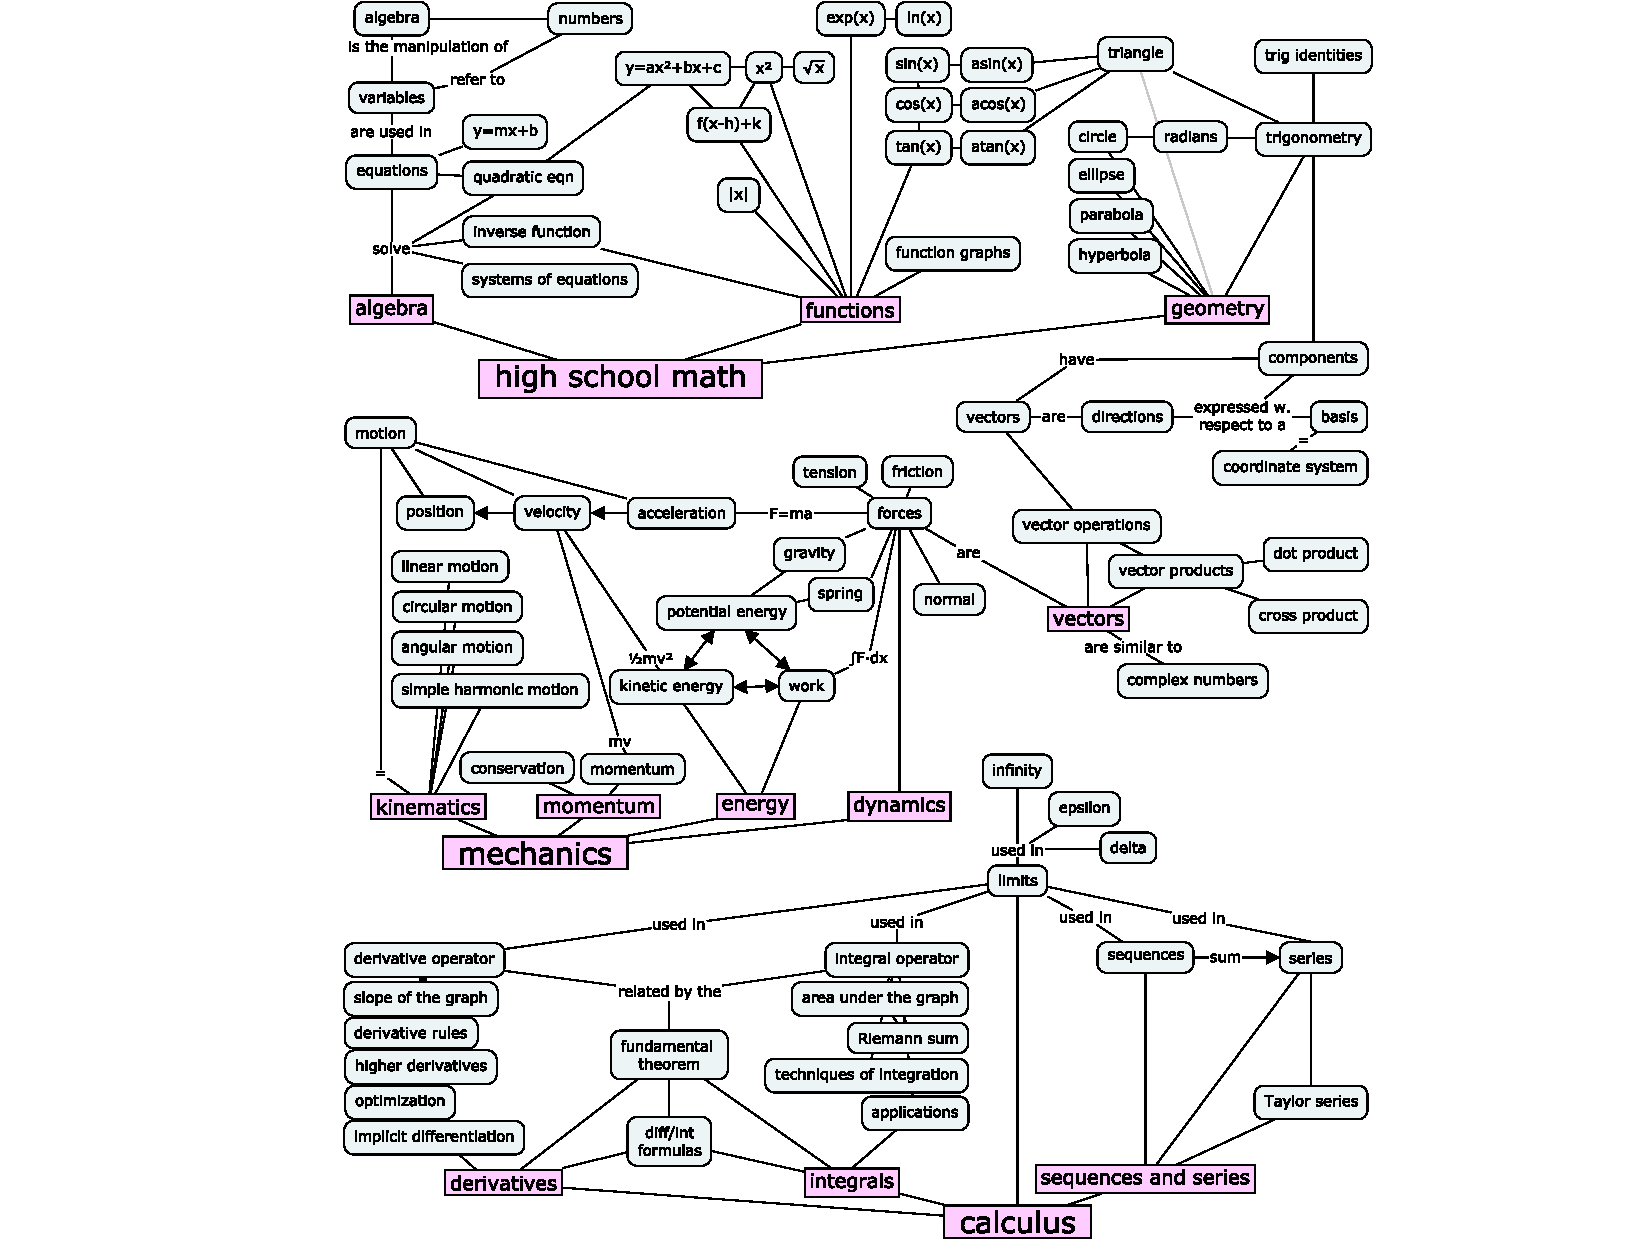
\includegraphics[width=1.06\textwidth]{figures/concept_maps/concept_map_full3.pdf}
	\caption{	This diagram shows the connections between the concepts, topics, and subjects covered in the book.
			Seeing the connections between concepts is key to understanding math and physics.}
	\label{fig:big_concept_map}
\end{figure}


\clearpage
\vspace*{5mm}
\noindent
You can annotate the concept map with your current knowledge of each concept to keep track of your progress through the book.
\begin{itemize}
	\item[--] Add a single dot ($\bullet$) next to all concepts you've heard of.
	\item[--] Add two dots ($\bullet\bullet$) next to concepts you think you know.
	\item[--] Add three dots ($\bullet\!\bullet\!\bullet$) next to concepts you've used in exercises and problems.
\end{itemize}
By collecting some dots every week,
you'll be able to move through the material in no time at all.

\bigskip
If you don't want to mark up your book,
you can download a printable version of the concept map here: 
\href{https://bit.ly/mathphyscmap}{\texttt{bit.ly/mathphyscmap}}.


\clearpage
\thispagestyle{plain}


%!TEX root = ../main.tex


%=======================================================================  preface
\chapter{Preface}
\label{sec:preface}

	This is a sample book project that showcases all the features and capabilities of the softcover eBook build system.

	\subsection{Why?}
	
		We should have a simple book example to show how the scripts work.
%%%%%%%%%%%%%%%%%%%%%%%%%%%%%%%%%%%%%%%%%%%%%%%%%%%%%%%%%%%%%%%%%%%%%%%


%%%   MAIN CONTENT    %%%%%%%%%%%%%%%%%%%%%%%%%%%%%%%%%%%%%%%%%%%%%%%%%%%%%%%%%
\mainmatter																			% start roman page numbering 
%!TEX root = ../main.tex


%=======================================================================  introduction
\softchapter{Introduction}
\label{sec:introduction}

	This is where the intro text would go.
	
	
	Below is an example figure.

	% MINI CHAPTER CONCEPT MAP
	\begin{figure}[htb]
		\centering
		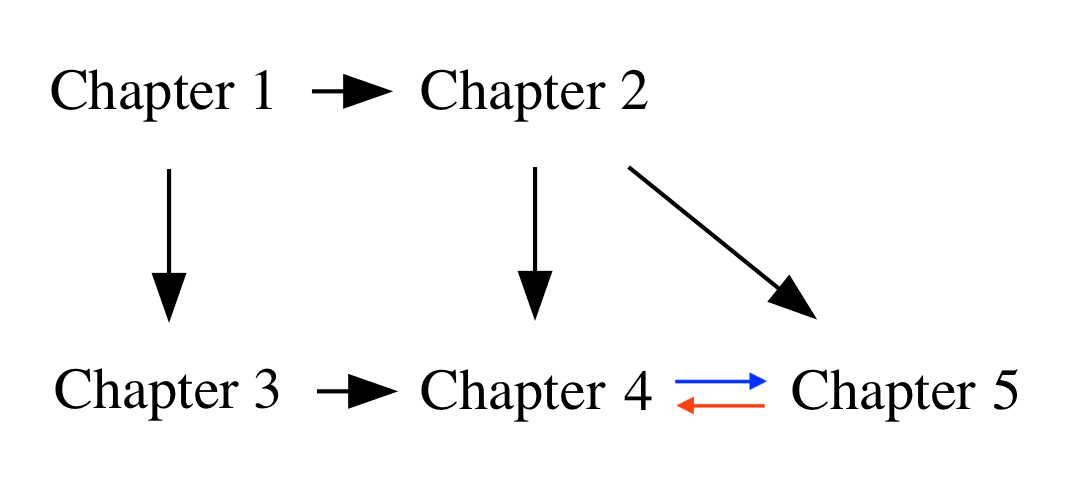
\includegraphics[width=0.58\textwidth]{figures/dot/chap_prereqs.png}
		\vspace{-3mm}
		\caption{The prerequisite structure for the chapters in this book.}
		\label{fig:chap_prereqs}
	\end{figure}


	Are you ready for this? Let's dig in!




%!TEX root = ../main.tex

%=============================================================================== 
%
%    Chapter: math_fundamentals
%
%=============================================================================== 

\chapter{Math fundamentals}
\label{chapter:math_fundamentals}

In this chapter we'll review the fundamental ideas of mathematics, including numbers, equations, and functions.  
To understand college-level textbooks, you need to be comfortable with mathematical calculations.
Many people have trouble with math, however. 
Some people say they \emph{hate} math, or could never learn it. 
It's not uncommon for children who score poorly on their school math exams to develop math complexes in their grown lives.
If you are carrying any such emotional baggage, you can drop it right here and right now.

Do NOT worry about math! 
You are an adult, and you can learn math much more easily than when you were a kid.
We'll review \emph{everything} you need to know about high school math, and by the end of this chapter, 
you'll see that math is nothing to worry about.

\smallskip

\begin{figure}[H]
\centering
\! 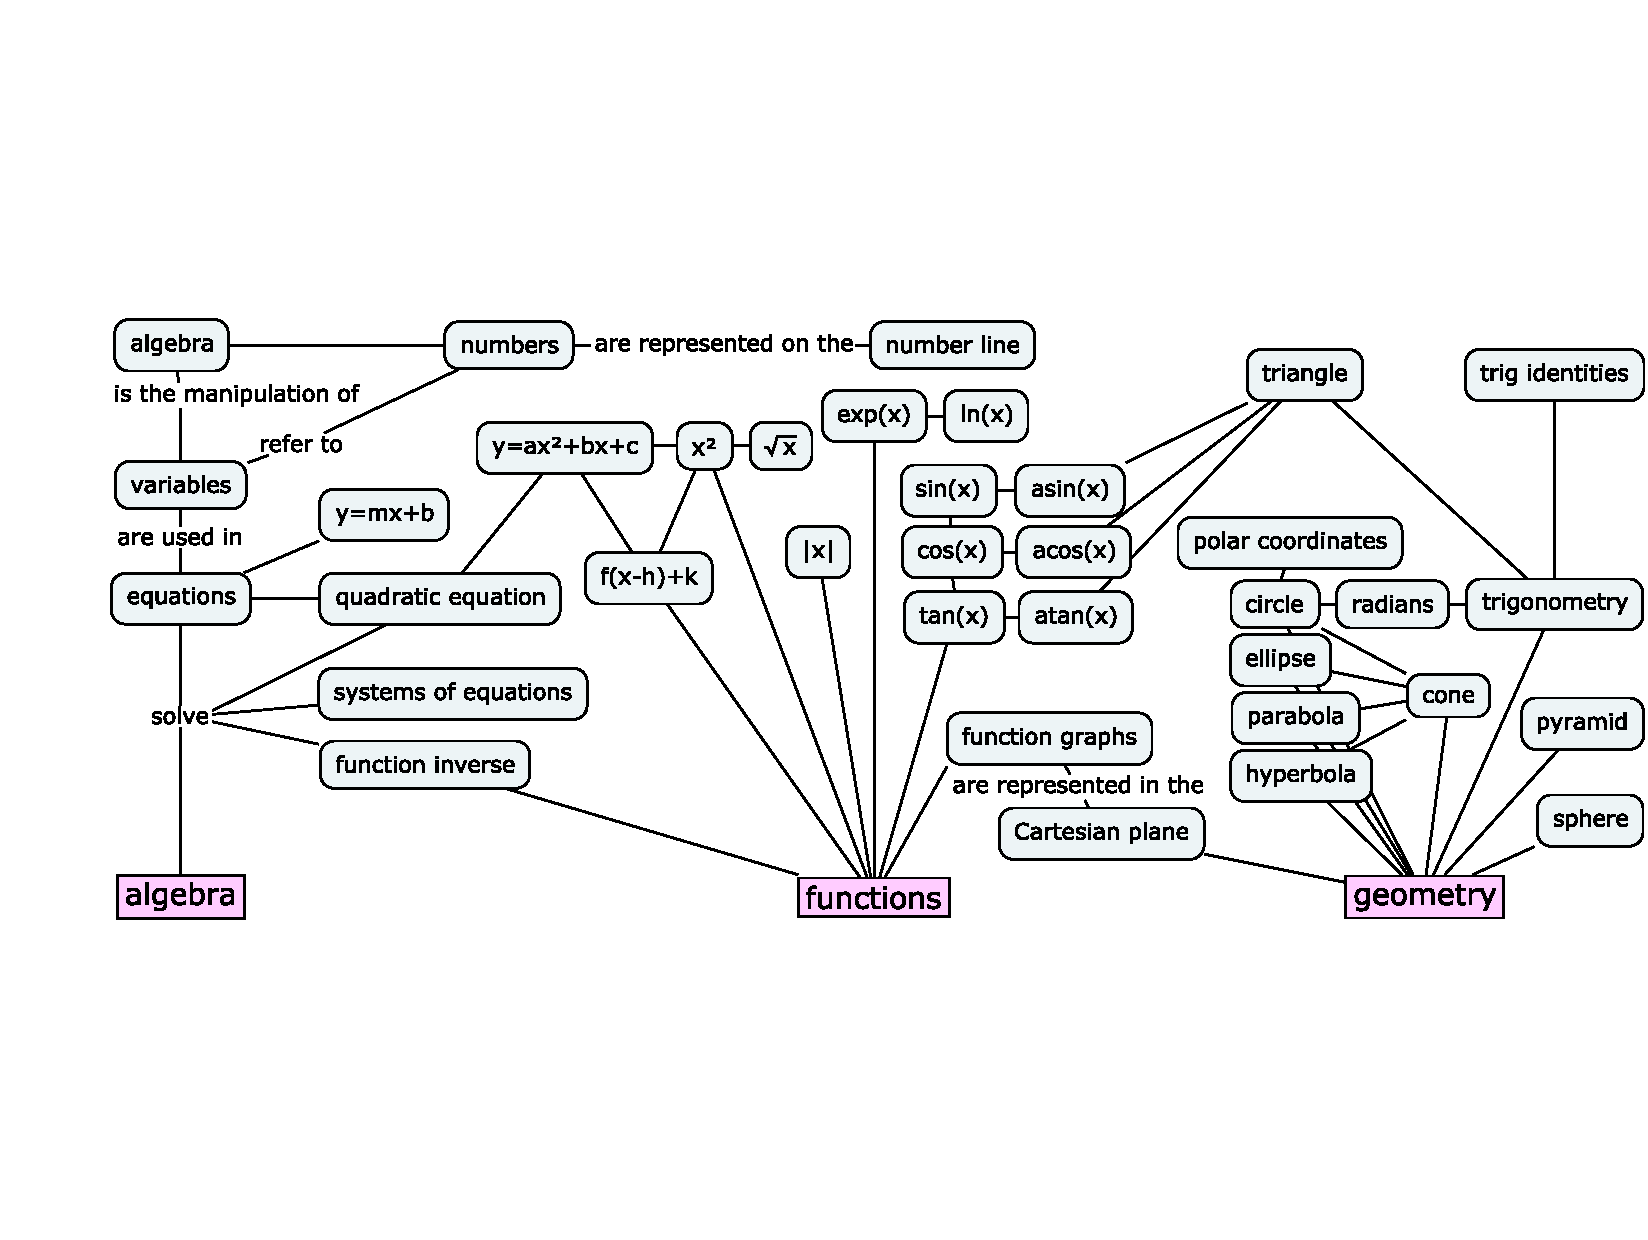
\includegraphics[width=1.01\textwidth]{figures/concept_maps/precalculus.pdf}
	\caption{A concept map showing the mathematical topics that we will cover in this chapter.
			We'll learn how to solve equations using algebra, 
			how to model the world using functions,
			and how to think geometrically.
			The material in this chapter is required for your understanding of the more advanced topics in this book.}
\label{fig:precalculus_concept_map}
\end{figure}

	\beforeFirstExercises{ch1}
	
%=======================================================================  solving_equations
\section{Solving equations}
\label{sec:solving_equations}
	
	Most math skills boil down to being able to manipulate and solve equations.
	Solving an equation means finding the value of the unknown in the equation.  

	Check this \pgt{}{shit} out:
	\[
	 x^2-4=45.
	\]
	To solve the above equation is to answer
	the question ``What is $x$?''
	More precisely, we want to find the number that can take the 
	place of $x$ in the equation so that the equality holds.
	In other words, we're asking,
	\[
	  \text{``Which number times itself minus four gives 45?''}
	\]
	That is quite a mouthful, don't you think? 
	To remedy this verbosity, mathematicians often use specialized symbols to describe math operations.
	The problem is that these specialized symbols can be very confusing. 
	Sometimes even the simplest math concepts are inaccessible if you don't know what the symbols mean. 

	What are your feelings about math, dear reader? Are you afraid of it? 
	Do you have anxiety attacks because you think it will be too difficult for you?
	Chill! Relax, my brothers and sisters. There's nothing to it.
	Nobody can magically guess the solution to an equation immediately.
	To find the solution, you must break the problem into simpler steps.
	Let's walk through this one together.

	To find $x$, we can manipulate the original equation, 
	transforming it into a different equation (as true as the first) that looks like this:
	\[
	  x \; = \textrm{ only numbers.}
	\]

	\noindent
	That's what it means to \emph{solve} an equation:
	the equation is solved because the unknown is isolated on one side,
	while the constants are grouped on the other side.
	You can type the numbers on the right-hand side into a calculator and obtain the numerical value of $x$.

	By the way, before we continue our discussion,
	let it be noted: the equality symbol ($=$) means that all that is to the left of $=$ 
	is equal to 
	all that is to the right of $=$. 
	To keep this equality statement true,  
	\textbf{for every change you apply to the left side of the equation, 
	you must apply the same change to the right side of the equation}.

	% Keeping that rule in mind,
	To find $x$,
	we need to manipulate the original equation into its final form,
	simplifying it step by step until it can't be simplified any further.
	The only requirement is that the manipulations we make transform one true equation into another true equation.
	In this example,
	the first simplifying step is to add the number four to both sides of the equation:
	\[
	 	x^2-4  \; + 4  	=	45    \; + 4, 	    \\
	\]
	which simplifies to
	\[
		x^2 	 		=	49.
	\]
	Now the expression looks simpler, yes?
	How did I know to perform this operation? 
	I wanted to ``undo'' the effects of the operation $-4$.
	We undo an operation by applying its \emphindexdef{inverse}.
	In the case where the operation is the subtraction of some amount,
	the inverse operation is the addition of the same amount.

	We're getting closer to our goal of \emph{isolating} $x$ on one side of the equation,							\index{isolate}
	leaving only numbers on the other side.
	The next step is to undo the square $x^2$ operation.
	The inverse operation of squaring a number $x^2$ is to take its square root $\sqrt{\phantom{a}\; }$,
	so that's what we'll do next. We obtain
	\[ 
	   \sqrt{x^2} 		= 	\sqrt{49}.
	\]
	Notice how we applied the square root  to both sides of the equation? 
	If we don't apply the same operation to both sides, we'll break the equality!

	The equation $\sqrt{x^2}= \sqrt{49}$ simplifies to 
	\[
	 	|x|	= 	7.
	 \]
	What's up with the vertical bars around $x$?
	The notation $|x|$ stands for the \emph{absolute value} of $x$,											\index{absolute value}
	which is the same as $x$ except we ignore the sign that indicates whether $x$ is positive or negative. 
	For example $|5|=5$ and $|-5|=5$, too.
	The equation $|x|=7$ indicates that both $x=7$ and $x=-7$ satisfy the equation $x^2 = 49$.
	Seven squared is 49, $7^2=49$, and negative seven squared is also 49, $(-7)^2 = 49$,
	because the two negative signs cancel each other out.

	The final solutions to the equation $x^2-4=45$ are													\index{solution set}
	\[
	 x  = 7 \qquad \textrm{and} \qquad   x=  - 7.
	\]
	Yes, there are \emph{two} possible answers. 
	You can check that both of the above values of $x$ satisfy the initial equation $x^2-4=45$.

	\bigskip

	If you are comfortable with all the notions of high school math
	and you feel you could have solved the equation $x^2-4=45$ on your own,		% TODOv6: special comment for readers who expected there to be two solutions
	then you can skim through this chapter quickly.
	If on the other hand you are wondering how the squiggle killed the power two,
	then this chapter is for you!
	In the following sections we will review all the essential concepts from
	high school math that you will need to power through the rest of this book.
	First, let me tell you about the different kinds of numbers.


	%!TEX root = ../main.tex

%=======================================================================  numbers
\section{Numbers}
\label{sec:numbers}

	In the beginning, we must define the main players in the world of math: numbers.

	\subsection{Definitions}
	\label{numbers:definitions}
		
		Numbers are the basic objects we use to count, measure, quantify, and calculate things.
		Mathematicians like to classify the different kinds of number-like objects into categories called \emph{sets}:					\index{set}
		\begin{itemize}
			\item  The natural numbers: $\mathbb{N} = \{0,1,2,3,4,5,6,7, \ldots \, \}$
			\item  The integers: $\mathbb{Z} = \{\ldots, -3,-2,-1,0,1,2,3 , \ldots  \, \}$
			\item  The rational numbers: $\mathbb{Q} = \{\frac{5}{3}, \frac{22}{7}, 1.5, 0.125,  -7, \, \ldots \, \}$
			\item  The real numbers: $\mathbb{R} = \{-1,0,1, \sqrt{2}, e,\pi, \;  4.94\ldots, \; \ldots \, \}$
			\item  The complex numbers: $\mathbb{C} = \{ -1, 0, 1, i,  1+i, 2+3i,  \ldots \, \}$
		\end{itemize}
		%
		These categories of numbers should be somewhat familiar to you.
		Think of them as neat classification labels for everything that you would normally call a number. 
	 	Each group in the above list is a \emph{set}.
		A set is a collection of items of the same kind. 
		Each collection has a name and a precise definition for which items belong in that collection.
		Note also that each of the sets in the list contains all the sets above it,												\index{set!subset}
		as illustrated in Figure~\ref{fig:nested_sets}.
		For now, we don't need to go into the details of \hyperref[sec:set_notation]{sets and set notation},
		but we do need to be aware of the different sets of numbers.

		\begin{figure}[H]
			\centering
			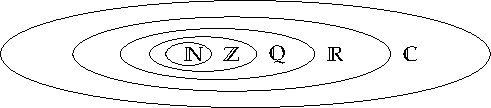
\includegraphics[width=0.87\textwidth]{figures/math/nested_sets.pdf}
			\caption{	An illustration of the nested containment structure of the different number sets.
					The set of natural numbers is contained in the set of integers,
					which in turn is contained in the set of rational numbers.
					The set of rational numbers is contained in the set of real numbers,
					which is contained in the set of complex numbers.}
			\label{fig:nested_sets}
		\end{figure}

		\noindent
		Why do we need so many different sets of numbers?
		Each set of numbers is associated with more and more advanced mathematical problems.

		The simplest numbers are the natural numbers $\mathbb{N}$,
		which are sufficient for all your math needs if all you're going to do is \emph{count} things.
		How many goats? Five goats here and six goats there so the total is 11 goats. 
		The sum of any two natural numbers is also a natural number.

		As soon as you start using \emph{subtraction} (the inverse operation of addition),
		you start running into negative numbers,
		which are numbers outside the set of natural numbers.
		If the only mathematical operations you will ever use are \emph{addition} and \emph{subtraction},
		then the set of integers $\mathbb{Z} = \{ \ldots, -2, -1, 0, 1, 2, \ldots \}$ will be sufficient.
		Think about it.
		Any integer plus or minus any other integer is still an integer.

		You can do a lot of interesting math with integers.
		There is an entire field in math called \emph{number theory} that deals with integers.
		However, to restrict yourself solely to integers is somewhat limiting---a rotisserie
		menu that offers $\frac{1}{2}$ of a chicken would be totally confusing.

		If you want to use division in your mathematical calculations,														\index{rational}
		you'll need the rationals~$\mathbb{Q}$.
		The set of rational numbers corresponds to all numbers that can be expressed as \emph{fractions} of the form $\frac{m}{n}$		\index{fraction}
		where $m$ and $n$ are integers, and $n \neq 0$.
		You can add, subtract, multiply, and divide rational numbers, and the result will always be a rational number.
		However, even the rationals are not enough for all of math!

		In geometry, we can obtain \emph{irrational} quantities like $\sqrt{2}$ (the diagonal of a square with side 1)
		and $\pi$ (the ratio between a circle's circumference and its diameter).
		There are no integers $x$ and $y$ such that $\sqrt{2}=\frac{x}{y}$,
		therefore we say that $\sqrt{2}$ is \emph{irrational} (not in the set $\mathbb{Q}$).
		An irrational number has an infinitely long decimal expansion that doesn't repeat.
		For example, $\pi = 3.141592653589793\ldots$ where the dots indicate
		that the decimal expansion of $\pi$ continues all the way to infinity.

		Combining the irrational numbers with the rationals gives us all the useful numbers,
		which we call the set of real numbers $\mathbb{R}$.
		The set $\mathbb{R}$ contains the integers,
		the rational numbers $\mathbb{Q}$,
		as well as irrational numbers like $\sqrt{2}=1.4142135\ldots$.
		By using the reals you can compute pretty much anything you want.
		From here on in the text, when I say \emph{number},
		I mean an element of the set of real numbers $\mathbb{R}$.

		The only thing you can't do with the reals is to take the square root of a negative number---you 							\index{complex number}
		need the complex numbers $\mathbb{C}$ for that.
		We defer the discussion on $\mathbb{C}$ until the end of Chapter~\ref{chapter:vectors}.


	\subsection{Exercises}
	\label{numbers:exercises}
	
		%!TEX root = ../main.tex

\begin{exercises}{ch1}	


	\begin{exercise}
		Solve for the unknown $x$ in the following equations:

		\twocol
		\textbf{a)}~$3x+2-5=4+2$

		\textbf{b)}~$\frac{1}{2}x-3=\sqrt{3}+12-\sqrt{3}$
		\endtwocol

		\twocol
		\textbf{c)}~$\frac{7x-4}{2} +1 = 8-2$
		
		\textbf{d)}~$5x-2+3=3x-5$
		\endtwocol
				
		\begin{eanswer}\textbf{a)}~$x=3$; \textbf{b)}~$x=30$; \textbf{c)}~$x=2$; \textbf{d)}~$x=-3$.\end{eanswer}
					\end{exercise}


	\begin{exercise}
		Indicate all the number sets the following numbers belong to.
				
		\fivecol
		\textbf{a)}~$-2$ 

		\textbf{b)}~$\sqrt{-3}$
		
		\textbf{c)}~$8 \div 4$
		
		\textbf{d)}~$\frac{5}{3}$
		
		\textbf{e)}~$\frac{\pi}{2}$
		
		\endfivecol
		
		\begin{eanswer}\textbf{a)}~$\mathbb{Z}, \mathbb{Q}, \mathbb{R},\mathbb{C}$;
					\textbf{b)}~$\mathbb{C}$;
					\textbf{c)}~$\mathbb{N},\mathbb{Z}, \mathbb{Q}, \mathbb{R},\mathbb{C}$;
					\textbf{d)}~$\mathbb{Q}, \mathbb{R},\mathbb{C}$;
					\textbf{e)}~$\mathbb{R},\mathbb{C}$.\end{eanswer}
					\end{exercise}

	

	\begin{exercise}
		Calculate the values of the following expressions:
		
		\threecol
		\textbf{a)}~$2^33-3$ 

		\textbf{b)}~$2^3(3-3)$
		
		\textbf{c)}~$\frac{4-2}{3^3}(6\cdot 7- 41)$
		\endthreecol
		
		\begin{eanswer}\textbf{a)}~$21$; \textbf{b)}~$0$; \textbf{c)}~$\frac{2}{27}$.\end{eanswer}
					\end{exercise}	



\end{exercises}

	


	%!TEX root = ../main.tex

%=======================================================================  hyperbola
\section{Hyperbola}
\label{sec:hyperbola}

	The \emphindexdef{hyperbola} is another fundamental shape of nature.
	

	\subsection{The conic sections}

		There is a deep connection between the geometric shapes of the circle,
		the ellipse, the parabola, and the hyperbola.
		These seemingly different shapes can be obtained, geometrically speaking,
		from a single object: the cone.															\index{cone}
		We can obtain the four curves by slicing the cone at different angles,
		as illustrated in Figure~\ref{fig:conic_sections_four-shapes}.

		\begin{figure}[htb]
			\centering
			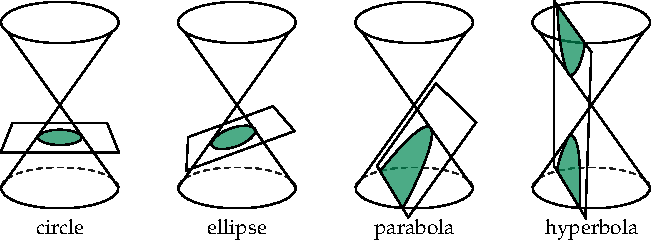
\includegraphics[width=0.8\textwidth]{figures/math/conic_sections_four-shapes.pdf}
			\vspace{-2mm}
			\caption{	Taking slices through a cone at different angles produces different geometric shapes:
					a circle, an ellipse, a parabola, or a hyperbola.}
			\label{fig:conic_sections_four-shapes}
		\end{figure}
	

	\subsection{Conic sections in polar coordinates}

		All four conic sections can be described by the same function in polar coordinates:					\index{polar coordinates}
		\[
		  r(\theta) = \frac{q(1+\varepsilon)}{1 + \varepsilon\cos(\theta)}\,,
		\]
		where $q$ is the curve's closest distance to a focal point
		and $\varepsilon$ is the curve's eccentricity.												\index{eccentricity}
		For a circle, $q=R$ (the radius) and the eccentricity parameter is $\varepsilon=0$.
		For an ellipse, $q=a(1-\varepsilon)$ and the eccentricity parameter varies between $0$ and $1$ ($0\leq \varepsilon < 1$).
		Note we include the case $\varepsilon=0$ since a circle is a special case of an ellipse.
		For a parabola, $q=f$ (the focal length) and the eccentricity is $\varepsilon=1$.
		For a hyperbola, $q = a(\varepsilon-1)$ and the eccentricity is $\varepsilon>1$.

		We can use the eccentricity parameter $\varepsilon$ to classify all four curves.
		Depending on the value of $\varepsilon$,
		the equation $r(\theta)$ defines either a circle, an ellipse, a parabola, or a hyperbola.	\index{circle}\index{ellipse}\index{hyperbola}\index{parabola}
		Table~\ref{table:conics} summarizes all our observations regarding conic sections.


		\begin{table}[htb]
		{ \small

		\centering 
		\begin{longtable}{@{}lllll@{}} 
		\toprule
		Conic section 	\! 	&  Equation  	\!\!					
		& Polar function	
		&	Eccentricity \!\!\!\!\!\!\!\!\!\!\!\!				\\
		\midrule
		Circle				& $x^2+y^2=R^2$ \; 					& $r(\theta)=R$			& $\varepsilon = 0$								\\[1mm]
		Ellipse				& $\frac{x^2}{a^2}+\frac{y^2}{b^2}=1$	& $r(\theta)=\frac{a(1-\varepsilon^2)}{1 + \varepsilon\cos(\theta)}$ &	$\varepsilon\!=\!\sqrt{1\!-\!\frac{b^2}{a^2}}\,, \; 0\!\leq\!\varepsilon\!<\!1$\!\!	\\[2mm]
		Parabola				& $y^2=4fx$						& $r(\theta)=\frac{2f}{1 + \cos(\theta)}$ &	$\varepsilon=1$			 						\\[1mm]
		Hyperbola			& $\frac{x^2}{a^2}-\frac{y^2}{b^2}=1$	& $r(\theta)=\frac{a(\varepsilon^2-1)}{1 + \varepsilon\cos(\theta)}$ &	$\varepsilon\!=\!\sqrt{1\!+\!\frac{b^2}{a^2}}\,, \; 1\!<\!\varepsilon\!<\!\infty$ \\[1mm]
		\bottomrule
		\end{longtable}

		}
		\vspace{4mm}
		\caption{The four conic sections and their eccentricity parameters. }
		\label{table:conics}
		\end{table}


		The motion of the planets is explained by Newton's law of gravitation.
		The gravitational interaction between two bodies always leads one of the two bodies to follow a trajectory described by one of the conic sections
		for which the other body is the focal point.

	\afterLastExercises{ch1}
	%!TEX root = ../main.tex


\section{Math problems}
\label{sec:math_problems}
	
	We've now reached the first section of problems in this book.
	The purpose of these problems is to give you a way to comprehensively practice your math fundamentals.

	
{\small 
	 
\begin{problems}{ch1}

	\vspace*{3mm}


	%%%  SOLVING EQUATIONS     %%%%%%%%%%%%%%%%%%%%%%%%%%%%%%%%%%%%
	
	\begin{problem}
		Solve for $x$ in the equation $x^2-9=7$.
		\begin{answer}$x=\pm 4$.\end{answer}
	\end{problem}

	\begin{problem}
		Solve for $x$ in the equation $\cos^{-1}\!\left( \frac{x}{A} \right) - \phi = \omega t$.
		\begin{answer}$x=A\cos(\omega t+\phi)$.\end{answer}
	\end{problem}

	\begin{problem}		\label{mathprob:ch1:fractions2}
		Solve for $x$ in the equation $\frac{1}{x}=\frac{1}{a}+\frac{1}{b}$.	
		\begin{answer}$x=\frac{ab}{a+b}$.\end{answer}
	\end{problem}

	\begin{problem}
		Use a calculator to find the values of the following expressions:
		\fourcol
			\textbf{a)}~$\sqrt[4]{3^3}$
			
			\textbf{b)}~$2^{10}$
			
			\textbf{c)}~$7^{^{\frac{1}{4}}}-10$
			
			\textbf{d)}~$\frac{1}{2}\ln(e^{22})$
		\endfourcol
		%\begin{hint}
		%\end{hint}
		\begin{answer}\textbf{a)}~$2.2795$.
					\textbf{b)}~$1024$.
					\textbf{c)}~$-8.373$.
					\textbf{d)}~$11$.\end{answer}
		%\begin{solution}
		%\end{solution}
	\end{problem}


	%% FRACTIONS    %%%%%%%%%%%%%%%%%%%%%%%%%%%%%%%%%%%%

	\begin{problem} 
		Compute the following expressions involving fractions:
		\threecol
			\textbf{a)}~$\dfrac{1}{2} + \dfrac{1}{4}$
			
			\textbf{b)}~$\dfrac{4}{7} - \dfrac{23}{5}$
			
			\textbf{c)}~$1\frac{3}{4} + 1\frac{31}{32}$
		\endthreecol
		\begin{answer}\textbf{a)}~$\frac{3}{4}$.
					\textbf{b)}~$\frac{-141}{35}$.
					\textbf{c)}~$3\frac{23}{32}$.\end{answer}
		\begin{solution}
			For \textbf{c)}, 
			$1\frac{3}{4} + 1\frac{31}{32} 
				= \frac{7}{4} + \frac{63}{32} 
				= \frac{56}{32} + \frac{63}{32} = \frac{119}{32}=3\frac{23}{32}$.
		\end{solution}
	\end{problem}

	
\end{problems}


} %/small






% The sample chapter from the original softcover book
\chapter{The first chapter}

\label{cha:a_chapter}

This is the first paragraph of the Softcover Markdown template produced with the \softcover\ command-line interface. It shows how to write a document in Markdown, a lightweight markup language, augmented with the \href{http://kramdown.gettalong.org/}{kramdown} converter and some custom extensions, including support for embedded \PolyTeX, a subset of the powerful \LaTeX\ typesetting system.\footnote{Pronunciations of {}``LaTeX{}'' differ, but \emph{lay}-tech is the one I prefer.} For more information, see \href{http://manual.softcover.io/book}{\emph{The Softcover Book}}. To learn how to easily publish (and optionally sell) documents produced with Softcover, visit \href{http://softcover.io/}{Softcover.io}.

This is the \emph{second} paragraph, showing how to emphasize text.\footnote{This is a footnote. It is numbered automatically.} You can also make text \textbf{bold} or \emph{emphasize a second way}. Via embedded \PolyTeX, Softcover also supports colored text, such as \coloredtext{red}{red}, \coloredtext{CornflowerBlue}{cornflower blue}, and \coloredtexthtml{E8AB3A}{arbitrary HTML colors}.

\section{A section}

\label{sec:a_section}

This is a section. You can refer to it using the \LaTeX\ cross-reference syntax, like so: Section~\ref{sec:a_section}.

\subsection{Source code}

This is a subsection.

You can typeset code samples and other verbatim text using four spaces of indentation:

\begin{verbatim}
def hello
  puts "hello, world"
end
\end{verbatim}

Softcover also comes with full support for syntax-highlighted source code using kramdown{}'s default syntax, which combines the language name with indentation:

%= lang:ruby
\begin{code}
def hello
  puts "hello, world"
end
\end{code}

Softcover{}'s Markdown mode also extends kramdown to support so-called {}``code fencing{}'' from GitHub-flavored Markdown:

%= lang:ruby
\begin{code}
def hello
  puts "hello, world!"
end
\end{code}

The last of these can be combined with \PolyTeX{}'s \kode{codelisting} environment to make code listings with linked cross-references (Listing~\ref{code:hello}).

\begin{codelisting}
\codecaption{Hello, world.}
\label{code:hello}
%= lang:ruby
\begin{code}
def hello
  puts "hello, world!"
end
\end{code}
\end{codelisting}

\subsection{Mathematics}

Softcover{}'s Markdown mode supports mathematical typesetting using \LaTeX\ syntax, including inline math, such as \( \phi^2 - \phi - 1 = 0, \) and centered math, such as
\[ \phi = \frac{1+\sqrt{5}}{2}. \]
It also supports centered equations with linked cross-reference via embedded \PolyTeX\ (Eq.~\eqref{eq:phi}).

\begin{equation}
\label{eq:phi}
\phi = \frac{1+\sqrt{5}}{2}
\end{equation}

Softcover also supports an alternate math syntax, such as \(\phi^2 - \phi - 1 = 0\), and centered math, such as

\[\phi = \frac{1+\sqrt{5}}{2}.\]

The \LaTeX\ syntax is strongly preferred, but the alternate syntax is included for maximum compatibility with other systems.

\section{Images and tables}

This is the second section.

Softcover supports the inclusion of images, like this:

\image{images/figures/conic_sections_four-shapes.png}

Using \LaTeX\ labels, you can also include a caption (as in Figure~\ref{fig:captioned_image}) or just a figure number (as in Figure~\ref{fig:figure_number}).

\begin{figure}[H]
\begin{center}
\image{images/figures/conic_sections_four-shapes.png}
\end{center}
\caption{The four conic sections.\label{fig:captioned_image}}

\end{figure}

\begin{figure}[H]
\begin{center}
\image{images/figures/conic_sections_four-shapes.png}
\end{center}
\caption{\label{fig:figure_number}}

\end{figure}

\subsection{Tables}

Softcover supports raw tables via a simple table syntax:

\begin{longtable}{|l|l|l|l|}
\hline
\textbf{HTTP request} & \textbf{URL} & \textbf{Action} & \textbf{Purpose}\\
\kode{GET} & /users & \kode{index} & page to list all users\\
\kode{GET} & /users/1 & \kode{show} & page to show user with id \kode{1}\\
\kode{GET} & /users/new & \kode{new} & page to make a new user\\
\kode{POST} & /users & \kode{create} & create a new user\\
\kode{GET} & /users/1/edit & \kode{edit} & page to edit user with id \kode{1}\\
\kode{PATCH} & /users/1 & \kode{update} & update user with id \kode{1}\\
\kode{DELETE} & /users/1 & \kode{destroy} & delete user with id \kode{1}\\
\hline
\end{longtable}

See \href{http://manual.softcover.io/book/softcover_markdown#sec-embedded_tabular_and_tables}{\emph{The Softcover Book}} to learn how to make more complicated tables.

\section{Command-line interface}

Softcover comes with a command-line interface called \kode{softcover}. To get more information, just run \kode{softcover help}:

%= lang:console
\begin{code}
$ softcover help
Commands:
  softcover build, build:all           # Build all formats
  softcover build:epub                 # Build EPUB
  softcover build:html                 # Build HTML
  softcover build:mobi                 # Build MOBI
  softcover build:pdf                  # Build PDF
  softcover build:preview              # Build book preview in all formats
  .
  .
  .
\end{code}

\noindent You can run \kode{softcover help \textless{}command\textgreater{}} to get additional help on a given command:

%= lang:console
\begin{code}
$ softcover help build
Usage:
  softcover build, build:all

Options:
  -q, [--quiet]   # Quiet output
  -s, [--silent]  # Silent output

Build all formats
\end{code}

\section{Miscellanea}

This is the end of the template---apart from two mostly empty chapters. In fact, let’s include the last chapter in its entirety, just to see how mostly empty it is:
%= <<(chapters/yet_another_chapter.tex, lang: text)

Visit \href{http://manual.softcover.io}{\emph{The Softcover Book}} to learn more about what Softcover can do.


%!TEX root = ../main.tex

%=============================================================================== 
%
%    Chapter: vectors
%
%=============================================================================== 

\chapter{Vectors}
\label{chapter:vectors}

In this chapter we'll learn how to manipulate multi-dimensional objects called vectors.						\index{vector|textbf}
Vectors are the precise way to describe directions in space.
We need vectors in order to describe physical quantities like forces, velocities, and accelerations.

Vectors are built from ordinary numbers,
which form the \emph{components} of the vector.
You can think of a vector as a list of numbers,
and \emph{vector algebra} as operations
performed on the numbers in the list.
Vectors can also be manipulated as geometric objects,
represented by arrows in space.
For instance, the arrow that corresponds to the vector $\vec{v}=(v_x,v_y)$ starts at the origin $(0,0)$
and ends at the point $(v_x,v_y)$.
The word vector comes from the Latin \emph{vehere},
which means \emph{to carry}.
Indeed, the vector $\vec{v}$ takes the point $(0,0)$ and carries it to the point $(v_x,v_y)$.

\begin{figure}[H]
	\centering
	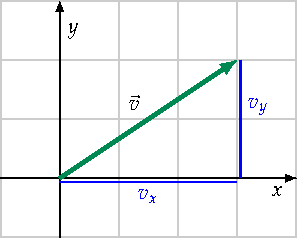
\includegraphics[width=0.4\textwidth]{figures/vectors/vector_components.pdf}
	\vspace{-2mm}
	\caption{	The vector $\vec{v}=(3,2)$ is an arrow in the Cartesian plane.
			The horizontal component of $\vec{v}$ is $v_x=3$
			and the vertical component  is $v_y=2$.}
	\label{fig:vector_components}
\end{figure}





	\beforeFirstExercises{ch3}
	%!TEX root = ../main.tex

%=======================================================================  vectors
\section{Vectors}
\label{sec:vectors}

	Vectors are extremely useful in all areas of life.
	In physics, for example, we use a vector to describe the velocity of an object.
	It is not sufficient to say that the speed of a tennis ball is 200 kilometres per hour:
	we must also specify the direction in which the ball is moving.
	Both of the two velocities 
	\[
	 \vec{v}_1 = (200,0) 
	 \qquad \textrm{and}
	 \qquad \vec{v}_2=(0,200)
	\]
	describe motion at the speed of $200$ kilometres per hour;
	but since one velocity points along the $x$-axis, and the other points along the $y$-axis,
	they are \emph{completely} different velocities. 
	The velocity vector contains information about the object's speed \emph{and} its direction.
	The direction makes a big difference.
	If it turns out the tennis ball is hurtling toward you, you'd better get out of the way!

	The main idea in this chapter is that \textbf{vectors are not the same as numbers}.
	We'll start by defining what vectors are.
	Then we'll describe all the mathematical operations we can perform with vectors,
	which include
		vector addition $\vec{u}+\vec{v}$, 
		vector subtraction $\vec{u}-\vec{v}$,
		vector scaling $\alpha\vec{v}$,
		and other operations.
	In Section~\ref{sec:vector_products} we'll also talk about two different kinds of vector products.


	\subsection{Definitions}
	\label{vectors:definitions}

		A two-dimensional vector $\vec{v}$ corresponds to a \emph{pair of numbers}:
		\[
			\vec{v} = (v_x, v_y),
		\]
		where $v_x$ is the \emph{$x$-component} of the vector and $v_y$ is its \emph{$y$-component}.					\index{components}
		We denote the set of two-dimensional vectors as $\mathbb{R}^2$,
		since the components of a two-dimensional vector are specified by two real numbers.
		We'll use the mathematical shorthand $\vec{v} \in \mathbb{R}^2$ to define a two-dimensional vector $\vec{v}$.
		Vectors in $\mathbb{R}^2$ can be represented as arrows in the Cartesian plane.
		See the vector $\vec{v}=(3,2)$ illustrated in Figure~\ref{fig:vector_components}.

		We can also define three-dimensional vectors like the vector $\vec{v} = (v_x, v_y, v_z) \in \mathbb{R}^3$,
		which has three components.
		Three-dimensional vectors can be represented as arrows in a coordinate system that has three axes,				\index{coordinate system!Cartesian}
		like the one shown in Figure~\ref{fig:empty_coordinate_system_3D} on page~\pageref{fig:empty_coordinate_system_3D}.
		A three-dimensional coordinate system is similar to the Cartesian coordinate system you're familiar with,
		and includes the additional $z$-axis that measures the height above the plane.
		In fact,
		there's no limit to the number of dimensions for vectors.
		We can define vectors in an $n$-dimensional space:								\index{dimension}
		$\vec{v} = (v_1, v_2, \ldots, v_n) \in \mathbb{R}^n$.
		For the sake of simplicity,
		we'll define all the vector operation formulas using two-dimensional vectors.
		Unless otherwise indicated in the text,
		all the formulas we give for two-dimensional vectors $\vec{v} \in \mathbb{R}^2$
		also apply to $n$-dimensional vectors $\vec{v} \in \mathbb{R}^n$.


		\subsubsection{Vector operations}

			Consider two vectors,
			$\vec{u}=(u_x,u_y) $ and $\vec{v}=(v_x,v_y)$,
			and assume that $\alpha \in \mathbb{R}$ is an arbitrary constant. 
			The following operations are defined for these vectors:
			\begin{itemize}
				\item 	\textbf{Addition:}	$\vec{u} + \vec{v} = (u_x+v_x,\, u_y+v_y)$
				\item 	\textbf{Subtraction:}	$\vec{u} - \vec{v} = (u_x-v_x,\, u_y-v_y)$
				\item 	\textbf{Scaling:}		$\alpha \vec{u} = (\alpha u_x,\, \alpha u_y)$
				\item 	\textbf{Dot product:}	$\vec{u} \cdot \vec{v}  = u_xv_x+u_yv_y$								\index{dot product}
				\item 	\textbf{Length:}		$\|\vec{u}\| = \sqrt{\vec{u}\cdot\vec{u}} = \sqrt{u_x^2+u_y^2}$.
						The vector's length is also called the \emph{norm} of the vector.
						We sometimes use the letter $u$ to denote the length of the vector $\vec{u}$.
			\end{itemize}

			\noindent
			Note there is no vector division operation.

			For vectors in a three-dimensional space $\vec{u}=(u_x,u_y,u_z) \in \mathbb{R}^3$
			and $\vec{v}=(v_x,v_y,v_z) \in \mathbb{R}^3$,
			we can also define the \textbf{cross product} operation												\index{cross product}
			$\vec{u} \times \vec{v} = (u_yv_z-u_zv_y,\; u_zv_x-u_xv_z,\; u_xv_y-u_yv_x)$.
			The dot product and the cross product are new operations that you probably haven't seen before.
			We'll talk more about dot products and the cross products in Section~\ref{sec:vector_products}.
			For now let's start with the basics.


		\subsubsection{Vector representations}

			We'll use three equivalent ways to denote vectors in two dimensions:
			\begin{itemize}
			    \item   	$\vec{v} =(v_x, v_y)$: component notation.
					The vector is written as a pair of numbers called the \emph{components} or \emph{coordinates} of the vector.	\index{coordinates}
			    \item 	$\vec{v} =v_x\hat{\imath}+ v_y\hat{\jmath}$: unit vector notation.
					The vector is expressed as a combination of the unit vectors
					$\hat{\imath} = (1,0)$ and $ \hat{\jmath} = (0,1)$.
			    \item   	$\vec{v}=\|\vec{v}\|\angle \theta$: length-and-direction notation (polar coordinates).
					The vector is expressed in terms of its \emph{length} $\|\vec{v}\|$
					and the angle $\theta$ that the vector makes with the $x$-axis.
			\end{itemize}

			\begin{figure}[htb]
				\centering
				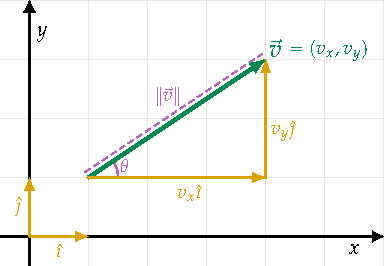
\includegraphics[width=0.6\textwidth]{figures/vectors/vector_components_annotated.pdf}
				\vspace{-2mm}
				\caption{The vector $\vec{v}=(v_x,v_y) = v_x\hat{\imath}+ v_y\hat{\jmath} = \|\vec{v}\|\angle \theta$.}
				\label{fig:vector_components_annotated}
			\end{figure}

			\noindent
			We use the component notation for doing vector algebra calculations since it is most compact.
			The unit vector notation shows explicitly that the vector $\vec{v}$ corresponds to the sum of
			$v_x\hat{\imath}$ (a displacement of $v_x$ steps in the direction of the $x$-axis)
			and $v_y\hat{\jmath}$ (a displacement of $v_y$ steps in the direction of the $y$-axis).
			The length-and-direction notation describes the vector $\vec{v}$
			as a displacement of $\|\vec{v}\|$ steps in the direction of the angle $\theta$.
			We'll use all three ways of denoting vectors throughout the rest of the book,
			and we'll learn how to convert between them.


	\subsection{Exercises}
	\label{basis:exercises}

		%!TEX root = ../main.tex

\begin{exercises}{ch3}

	\begin{exercise}
		Given the vectors $\vec{v}_1=(2,1)$, $\vec{v}_2=(2,-1)$, and $\vec{v}_3=(3,3)$,
		calculate the following expressions:
		\threecol
			\textbf{a)}~$\vec{v}_1 + \vec{v}_2$
			
			\textbf{b)}~$\vec{v}_2 - 2\vec{v}_1$
			
			\textbf{c)}~$\vec{v}_1 + \vec{v}_2 + \vec{v}_3$
		\endthreecol
		
		\begin{eanswer}\textbf{a)}~$(4,0)$.
					\textbf{b)}~$(-2,-3)$.
					\textbf{c)}~$(7,3)$.\end{eanswer}
	\end{exercise}

	\begin{exercise}	\label{exercise:vector-polar-to-cartesian-conversion}
		Express the following vectors as components:
		\threecol
			\textbf{a)}~$\vec{v}_1 =10\angle30^\circ$
			
			\textbf{b)}~$\vec{v}_2 = 12\angle\!-\!90^\circ$
			
			\textbf{c)}~$\vec{v}_3 = 3\angle170^\circ$
		\endthreecol

		\begin{eanswer}\textbf{a)}~$\vec{v}_1=(5\sqrt{3},5)=(8.66,5)$.
					\textbf{b)}~$\vec{v}_2=(0,-12)$.
					\textbf{c)}~$\vec{v}_3=(-2.95,0.52)$.\end{eanswer}
	\end{exercise}


	\begin{exercise}	\label{exercise:vector-cartesian-to-polar-conversion}
		Express the following vectors in length-and-direction notation:
		\threecol
			\textbf{a)}~$\vec{u}_1 = (4,0)$
			
			\textbf{b)}~$\vec{u}_2 = (1,1)$
			
			\textbf{c)}~$\vec{u}_3 = (-1,3)$
		\endthreecol

		\begin{eanswer}\textbf{a)}~$\vec{u}_1=4\angle 0^\circ$. 
					\textbf{b)}~$\vec{u}_2=\sqrt{2}\angle 45^\circ$.
					\textbf{c)}~$\vec{u}_3=\sqrt{10}\angle108.43^\circ$.\end{eanswer}
	\end{exercise}



%		Express the following vectors in terms of unit vectors $\hat{\imath}$, $\hat{\jmath}$, and $\hat{k}$:		%		\threecol
%			
%			
%		\endthreecol
%		\begin{eanswer}\textbf{a)}~$\vec{w}_1=9.06\hat{\imath}  + 4.23\hat{\jmath}$.
%					\textbf{c)}~$\vec{w}_3=7\hat{\imath}  +6 \hat{\jmath} + 5\hat{k}$.\end{eanswer}




\end{exercises}



	\afterLastExercises{ch3}
	%!TEX root = ../main.tex

\section{Vectors problems}
\label{sec:vec_problems}

\vspace{-2mm}

You learned a bunch of vector formulas and you saw some vector diagrams,
but did you really learn how to solve problems with vectors?
There is only one way to find out: test yourself by solving problems.

I've said it before and I don't want to repeat myself too much,
but it's worth saying again: the more problems you solve, the better you'll understand the material.
It's now time for you to try the following vector problems to make sure you're on top of things.

\medskip

{ \small

\begin{problems}{ch3}

	\begin{problem}
		Given the vectors $\vec{u}=(1,1,1)$, $\vec{v} = (2,3,1)$, and $\vec{w}=(-1,-1,2)$,
		compute the following products:
		
		\threecol
			\textbf{a)}~$\vec{u} \cdot \vec{v}$

			\textbf{b)}~$\vec{u} \cdot \vec{w}$
			
			\textbf{c)}~$\vec{v} \cdot \vec{w}$
		\endthreecol
		
		\threecol
			\textbf{d)}~$\vec{u} \times \vec{v}$

			\textbf{e)}~$\vec{u} \times \vec{w}$
			
			\textbf{f)}~$\vec{v} \times \vec{w}$
		\endthreecol
		
		\begin{answer}\textbf{a)}~$6$.
					\textbf{b)}~$0$.
					\textbf{c)}~$-3$.
					\textbf{d)}~$(-2, 1, 1)$.
					\textbf{e)}~$(3, -3, 0)$.
					\textbf{f)}~$(7, -5, 1)$.\end{answer}
	\end{problem}


	\begin{problem}
		Given the vectors $\vec{p} =(1,1,0,3,3)$ and $\vec{q}=(1,2,3,4,5)$, calculate the following expressions:
		\threecol
			\textbf{a)}~$\vec{p}+\vec{q}$
			
			\textbf{b)}~$\vec{p}-\vec{q}$
			
			\textbf{c)}~$\vec{p} \cdot \vec{q}$
		\endthreecol
		
		\begin{answer}\textbf{a)}~$(2,3,3,7,8)$.
					\textbf{b)}~$(0,-1,-3,-1,-2)$.
					\textbf{c)}~$30$.\end{answer}
	\end{problem}


	\begin{problem}
		Find a unit vector that is perpendicular to both  $\vec{u}=(1, 0, 1)$ and $\vec{v} =(1, 2, 0)$.
		\begin{hint}
			Use the cross product.
		\end{hint}
		\begin{answer}$(-\frac{2}{3}, \frac{1}{3}, \frac{2}{3})$ or $(\frac{2}{3}, -\frac{1}{3}, -\frac{2}{3})$.\end{answer}
		\begin{solution}See \href{http://bit.ly/1cOa8yo}{\texttt{bit.ly/1cOa8yo}} for calculations.
		\end{solution}
	\end{problem}

	\begin{problem}
		Find a vector that is orthogonal to both $\vec{u}_1 = (1, 0, 1)$ and $\vec{u}_2 =(1, 3, 0)$, 
		 and whose dot product with the vector  $\vec{v}= (1, 1, 0)$ is equal to $8$.
		%	\begin{hint}
		%	\end{hint}
		\begin{answer}$(12, -4, -12)$.\end{answer}
		\begin{solution}
			Any multiple of the vector $\vec{u}_1 \times \vec{u}_2 = (-3,1,3)$ 
			is perpendicular to both $\vec{u}_1$ and 	$\vec{u}_2$.
			We must find a multiplier $t \in \mathbb{R}$ such that 
			$t(-3,1,3) \cdot (1, 1, 0) = 8$.
			Computing the dot product we find $-3t + t = 8$, so $t=-4$.
			The vector we're looking for is $(12, -4, -12)$.
			See \href{http://bit.ly/1nmYH8T}{\texttt{bit.ly/1nmYH8T}} for calculations.
		\end{solution}
	\end{problem}


\end{problems}

} % /small



%%%%%%%%%%%%%%%%%%%%%%%%%%%%%%%%%%%%%%%%%%%%%%%%%%%%%%%%%%%%%%%%%%%%%%%


%%   END MATTER   %%%%%%%%%%%%%%%%%%%%%%%%%%%%%%%%%%%%%%%%%%%%%%%%%%%%%%%%%%%
%!TEX root = ../main.tex

%=============================================================================== 
%
%    Chapter: end_matter
%
%=============================================================================== 

\softchapter{End matter}
\label{chaptxer:end_matter}


%=======================================================================  conclusion
\softsection{Conclusion}
\label{sec:conclusion}

	This is where the conclusion would go.


%=======================================================================  acknowledgments
\softsection{Acknowledgments}
\label{sec:acknowledgments}
	
	This book would not have been possible without the support and encouragement of the people around me.
	I am fortunate to have grown up surrounded by good people who knew the value of math
	and encouraged me in my studies and with this project.
	In this section, I want to \emph{big up} all the people who deserve it.


%%=======================================================================  further_reading
\softsection{Further reading}
\label{sec:further_reading}

	You have reached the end of this book,
	but you're only at the beginning of the journey of scientific discovery.
	There are a lot of cool things left for you to learn about.
	Below are some recommendation of subjects you might find interesting.

\appendix 
%!TEX root = ../main.tex

\chapter{Answers and solutions}
\label{appendix:ans_and_solutions}

%\def\cleardoublepage{\clearpage}		% Appendices open on left OK 

\setlength\partopsep{-0.5\topsep}   % so solutions environments appear w/o space between them
%\setlength\partopsep{-\topsep}
%\addtolength\partopsep{-\parskip}


	\section*{Chapter 1 solutions}
	\label{sec:chapter1sols}	
	{ \footnotesize 

		\subsection*{Answers to exercises}
		\showExerciseAnswers{ch1}

		\subsection*{Solutions to selected exercises}
		\showExerciseSolutions{ch1}
		
		\subsection*{Answers to problems}
		\showProblemAnswers{ch1}

		\subsection*{Solutions to selected problems}
		\showProblemSolutions{ch1}

	}  % /footnotesize


	\section*{Chapter 2 solutions}
	\label{sec:chapter1sols}	
	{ \footnotesize 

		\subsection*{Answers to exercises}
		\showExerciseAnswers{ch2}

		\subsection*{Solutions to selected exercises}
		\showExerciseSolutions{ch2}
		
		\subsection*{Answers to problems}
		\showProblemAnswers{ch2}

		\subsection*{Solutions to selected problems}
		\showProblemSolutions{ch2}

	}  % /footnotesize



	\section*{Chapter 3 solutions}
	\label{sec:chapter3sols}	
	{ \footnotesize 

		\subsection*{Answers to problems}
		\showProblemAnswers{ch3}

		\subsection*{Solutions to selected problems}
		\showProblemSolutions{ch3}

	}  % /footnotesize


%!TEX root = ../main.tex

\chapter{Notation}
\label{appendix:notation}
\vspace{-7mm}

This appendix contains a summary of the notation used in this book.


\softsection{Math notation}

{ \small
\noindent
\begin{tabularx}{\textwidth}{@{}rlp{5.9cm}@{}} 
\toprule
Expression  	&	Read as  	& Used to denote			\\
\midrule
$a,b,x,y$	
	& 
	& variables \\
$=$	
	& is equal to 
	& expressions that have the same value \\ % have the same value	\\
$\eqdef$
	& is defined as 
	& a new variable definition  \\
$a+b$
	& $a$ plus $b$
	& the combined lengths of $a$ and $b$ \\
$a-b$	
	& $a$ minus $b$
	& the difference in lengths between $a$ and $b$ \\
$a\times b = ab$
	& $a$ times $b$
	& the area of a rectangle   \\
$a^2= aa$
	& $a$ squared 
	& the area of a square of side length $a$ \\
$a^3= aaa$
	& $a$ cubed 
	& the volume of a cube of side length $a$ \\
$a^n$
	& $a$ to the $n$
	%raised to the $n$\textsuperscript{th} power
	& $a$ multiplied by itself $n$ times 		\\
$\sqrt{a} = a^{\frac{1}{2}}$
	& square root of $a$
	& the side length of a square of area $a$ \\
$\sqrt[3]{a}= a^{\frac{1}{3}}$
	& cube root of $a$
	& the side length of a cube with volume $a$  \\
$a/b = \frac{a}{b}$
	& $a$ divided by $b$
	& $a$ parts of a whole split into $b$ parts \\[0.8mm]
$a^{-1}= \frac{1}{a}$
	& one over $a$
	& division by $a$ 					\\[2mm]
$f(x)$	
	& $f$ of $x$
	& the function $f$ applied to input $x$ 	\\
$f^{-1}$ 
	& $f$ inverse 
	& the inverse function of $f(x)$   \\
$f \circ g$ 
	& $f$ compose $g$ 
	& function composition; $f \circ g(x) = f(g(x))$   \\[2mm]
$e^x$ 
	& $e$ to the $x$ 
	& the exponential function base $e$ \\
$\ln(x)$ 
	& natural log of $x$ 
	& the logarithm base $e$ 				\\
$a^x$ 
	& $a$ to the $x$ 
	& the exponential function base $a$ \\
$\log_a(x)$ 
	& log base $a$ of $x$ 
	& the logarithm base $a$ 				\\[2mm]
$\theta,\phi$
	& \emph{theta}, \emph{phi}
	& angles 					\\
$\sin,\cos,\tan$
	& sin, cos, tan 
	& trigonometric ratios 			\\
%\; \\
$\%$
	& percent
	& proportions of a total; $a\%=\frac{a}{100}$ 		\\
\bottomrule
\end{tabularx}
}%

%%%%%%%%%%%%%%%%%%%%%%%%%%%%%%%%%%%%%%%%%%%%%%%%%%%%%%%%%%%%%%%%%%%%%%


%%   INDEX   %%%%%%%%%%%%%%%%%%%%%%%%%%%%%%%%%%%%%%%%%%%%%%%%%%%%%%%%%%%%%%%
{ \small
	\indexprologue{
		\label{thebookindex}
		\noindent
		The page numbers shown in \textbf{bold} point to the concept definitions.
	}
	\printindex
}
%%%%%%%%%%%%%%%%%%%%%%%%%%%%%%%%%%%%%%%%%%%%%%%%%%%%%%%%%%%%%%%%%%%%%%


    
        
\end{document}
%%%%%%%%%%%%%%%%%%%%%%%%%%%%%%%%%%%%%%%%%%%%%%%%%%%%%%%%%%%%%%%%%%%%%%%
